\documentclass[preprint,10pt,numbers]{sigplanconf}

% The following \documentclass options may be useful:

% preprint      Remove this option only once the paper is in final form.
% 10pt          To set in 10-point type instead of 9-point.
% 11pt          To set in 11-point type instead of 9-point.
% numbers       To obtain numeric citation style instead of author/year.

\usepackage{amsmath}
\usepackage{amsfonts}
\usepackage{listings}
\usepackage{color}
\usepackage[dvipsnames]{xcolor}
\usepackage{xspace}
\usepackage{comment}
\usepackage{graphicx} 
\usepackage{inconsolata}
\usepackage{appendix}
\usepackage{wrapfig}
\usepackage{multirow}
\usepackage{bm}
\usepackage{microtype}

\definecolor{listinggreen}{rgb}{0,0.6,0}
\definecolor{listinggray}{rgb}{0.5,0.5,0.5}
\definecolor{listingmauve}{rgb}{0.58,0,0.82}
\definecolor{listingkeywordcolor}{rgb}{1.0,0.4,0.0}
\definecolor{listinglightgray}{rgb}{0.8863,0.8863,0.8863}

\newcommand\layeronecolor{blue}

\newcommand\TODO[1]{{\color{red}\textbf{TODO: }#1}}
\newcommand\TOSAY[1]{{\color{black}\textbf{We Should Say That: }#1}}
\newcommand\COMMENT[1]{}
\newcommand\framework{\textsc{Tiramisu}\xspace}
\newcommand\processor{processor\xspace}
\newcommand\Processor{Processor\xspace}
\newcommand\layerone{abstract computation layer\xspace}
\newcommand\Layerone{Abstract Computation Layer\xspace}
\newcommand\layertwo{computation placement layer\xspace}
\newcommand\Layertwo{Computation Placement Layer\xspace}
\newcommand\layerthree{concrete computation layer\xspace}
\newcommand\Layerthree{Concrete Computation Layer\xspace}
%\newcommand\id[2]{{\color{Red} #1} : {\color{black} #2}}
%\newcommand\tsd[2]{{\color{Red} #1} : {\color{black} #2}}
%\newcommand\data[1]{{\color{PineGreen} #1}}
\newcommand{\pgrammar}[1]{\text{\sf\textless#1\textgreater}}

\newcommand\codeone{(a)\xspace}
\newcommand\codeonebis{(b)\xspace}
\newcommand\codetwo{(c)\xspace}
\newcommand\codethree{(d)\xspace}
\newcommand\codefour{(e)\xspace}

\lstset{ %
  backgroundcolor=\color{white},   % choose the background color; you must add \usepackage{color} or \usepackage{xcolor}
  basicstyle=\linespread{0.7}\footnotesize\ttfamily,        % the size of the fonts that are used for the code (scriptsize will violate min font size for PLDI)
  columns=fullflexible,
  breakatwhitespace=false,         % sets if automatic breaks should only happen at whitespace
  breaklines=true,                 % sets automatic line breaking
  captionpos=none,                 % sets the caption-position to bottom
  commentstyle=\color{listinggreen},% comment style
  deletekeywords={...},            % if you want to delete keywords from the given language
  escapeinside={\%*}{*)},          % if you want to add LaTeX within your code
  extendedchars=true,              % lets you use non-ASCII characters; for 8-bits encodings only, does not work with UTF-8
  frame=none,                      % adds a frame around the code
  keepspaces=true,                 % keeps spaces in text, useful for keeping indentation of code (possibly needs columns=flexible)
  keywordstyle=\color{listingkeywordcolor}\bfseries,       % keyword style
  language=C,             % the language of the code
  morekeywords={*,...},            % if you want to add more keywords to the set
  numbers=left,                    % where to put the line-numbers; possible values are (none, left, right)
  numbersep=5pt,                   % how far the line-numbers are from the code
  numberstyle=\tiny\color{listinggray}, % the style that is used for the line-numbers
  rulecolor=\color{black},         % if not set, the frame-color may be changed on line-breaks within not-black text (e.g. comments (green here))
  showspaces=false,                % show spaces everywhere adding particular underscores; it overrides 'showstringspaces'
  showstringspaces=false,          % underline spaces within strings only
  showtabs=false,                  % show tabs within strings adding particular underscores
  stepnumber=1,                    % the step between two line-numbers. If it's 1, each line will be numbered
  stringstyle=\color{listingmauve},% string literal style
  tabsize=2,                       % sets default tabsize to 2 spaces
  title=\lstname                   % show the filename of files included with \lstinputlisting; also try caption instead of title
}


\newcommand{\cL}{{\cal L}}











\begin{document}

\special{papersize=8.5in,11in}
\setlength{\pdfpageheight}{\paperheight}
\setlength{\pdfpagewidth}{\paperwidth}

\conferenceinfo{PLDI '17}{June 18--23, 2017, Barcelona, Spain}
\copyrightyear{2017}
\copyrightdata{978-1-nnnn-nnnn-n/yy/mm}
\copyrightdoi{nnnnnnn.nnnnnnn}

% Uncomment the publication rights you want to use.
%\publicationrights{transferred}
%\publicationrights{licensed}     % this is the default
%\publicationrights{author-pays}

\titlebanner{}        % These are ignored unless
\preprintfooter{}   % 'preprint' option specified.

%\title{\TODO{Change title}\framework{}: a Framework for Iteration Space Transformation Separating the Algorithm, the Schedule and the Data-layout}
\title{\framework{}: Polyhedral-Based Mid-Level Compiler for Domain Specific Languages}
\subtitle{}

\authorinfo{}
           {}
           {}
%\authorinfo{Name2\and Name3}
%           {Affiliation2/3}
%           {Email2/3}

\maketitle

\begin{abstract}

Compilers for high performance domain-specific languages (DSLs) are becoming more common,
due to their demonstrated ability to leverage domain-specific optimizations to transform
user code into high performance executables.  These optimizations
mostly transform high-level code to enable high performance execution in multicores and graphics processing
units (GPUs). However, state-of-the-art back-end compilers such as LLVM do not optimize beyond a single core with vector units.  Thus, DSL compilers need to expand into \emph{middle-end} compilers to enable these architectural optimizations,
and most DSL compilers re-implement the same set of middle-end optimizations.  In this paper,
we introduce \framework{}, a common middle-end compiler and representation suitable as a
target for DSL compilers.  \framework{} introduces a three-level representation that separates the
algorithm, how that algorithm is executed, and where intermediate data are stored.  As a result,
DSL compilers can be made considerably less complex with no loss of performance.  We evaluate
\framework by creating a new middle-end for the Halide compiler, and demonstrate no loss of performance
while reducing the amount of middle-end code substantially.  Finally, we also demonstrate
transformations made possible by \framework that are not possible in Halide, increasing performance
by up to $10\times$.

\end{abstract}

\category{D.3.4}{Programming Languages}{Processors -- compilers, optimization,
code generation}

% general terms are not compulsory anymore,
% you may leave them out
%\terms
%term1, term2

\keywords
intermediate representation; domain specific language; polyhedral
compilation; iteration space transformation; parallelism;
vectorization; GPU


\vspace{-0.25cm}
\section{Introduction}
\label{sec:intro}

Generating efficient code for high performance systems is becoming more and more difficult as these architectures are increasing in complexity and diversity.
Obtaining the best performance requires complex code and data layout transformations, management of complex memory hierarchies, and efficient data communication and synchronization.

For example, consider generalized matrix multiplication (\texttt{gemm}), which computes $C = \alpha AB + \beta C$ and is a
building block of numerous algorithms, including simulations and convolutional neural networks.  Highly-tuned implementations
require fusing the multiplication and addition loops, as well as applying two-level tiling, vectorization, loop unrolling, array packing~\cite{Goto:2008:AHM:1356052.1356053},
register blocking, and data prefetching.  Furthermore, tuned implementations separate partial tiles from full tiles, since partial tiles cannot fully benefit from the same optimizations.
High performance GPU implementations require even more optimizations.  Memory accesses should be coalesced, and data movement must be managed between global memory, shared memory, and registers, with synchronization primitives inserted where necessary.
Automatically generating such complex code is still beyond the capabilities of state-of-the-art compilers.
The importance of kernels such as \texttt{gemm}, along with the immense complexity of optimized implementations, motivate vendors to release highly hand-optimized libraries for such kernels.  However, for most users, obtaining this level of performance for their own code is challenging, since the effort required to explore the space of possible implementations is intractable when hand-coding complex code transformations.

\begin{figure}[t]
\centering
  \begin{minipage}{0.22\textwidth}
    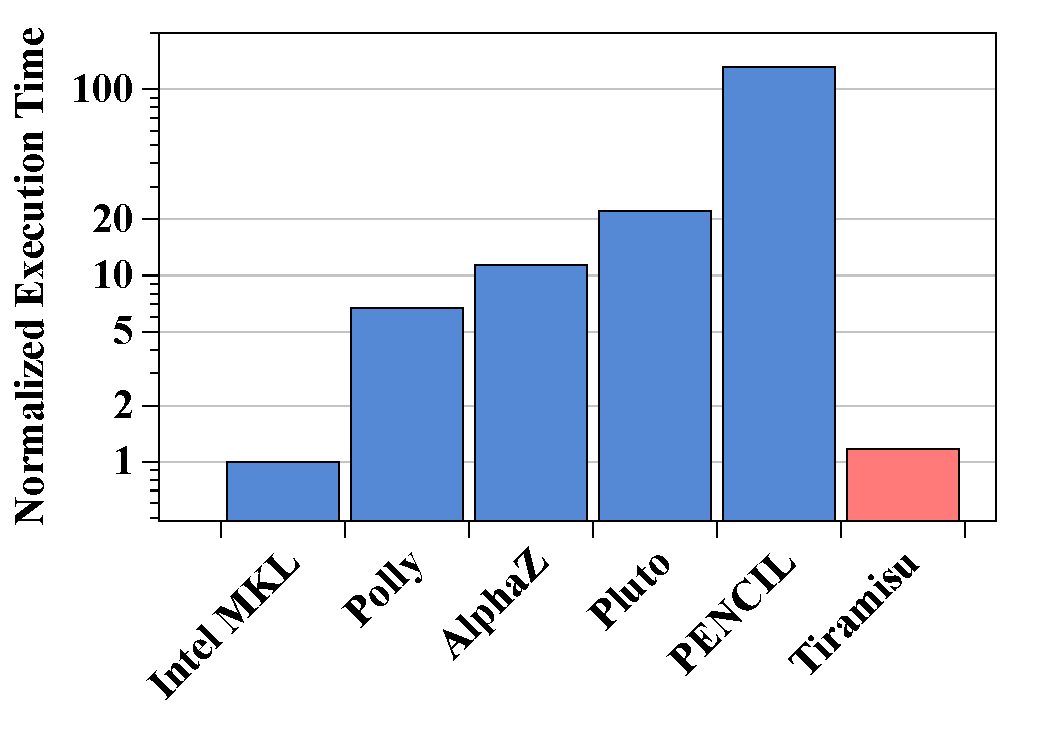
\includegraphics[width=\columnwidth]{./figures/sgemm_performance_CPU.pdf}
  \end{minipage}
  \begin{minipage}{0.22\textwidth}
    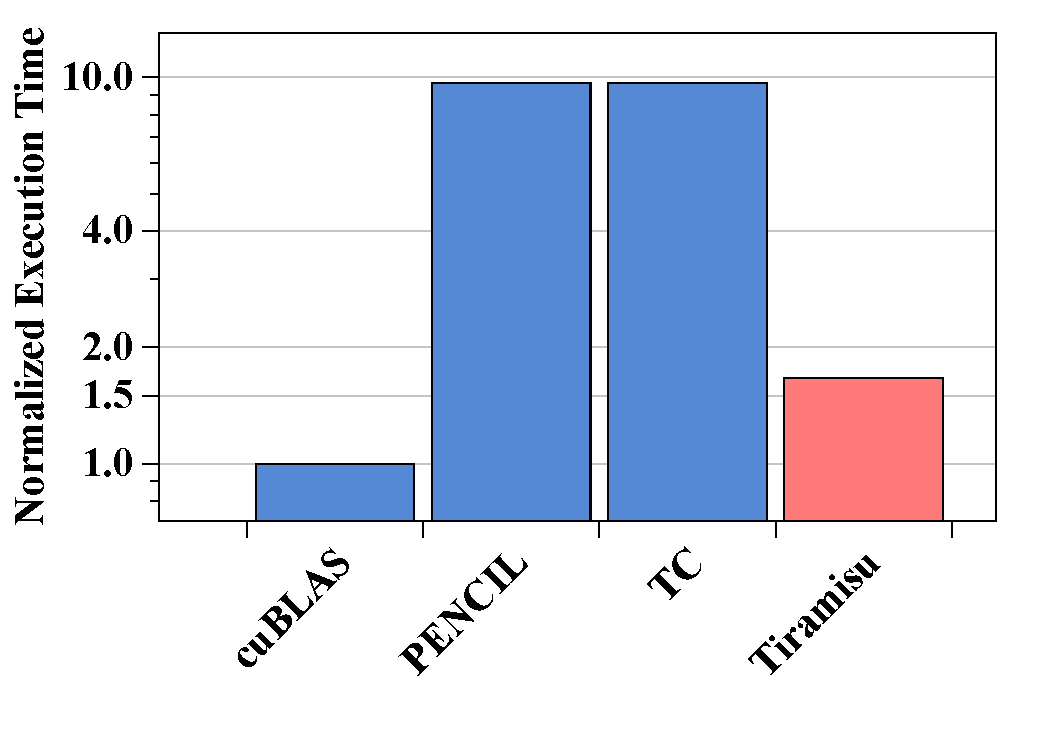
\includegraphics[width=\columnwidth]{./figures/sgemm_performance_GPU.pdf}
  \end{minipage}
  \vspace{-0.5cm}
  \caption{Normalized execution times of code generated for \texttt{sgemm} on CPU (left) and GPU (right).}
  \label{gemm-cpu-gpu}
  \vspace{-0.5cm}
\end{figure}

Previous work using the polyhedral model has shown success in implementing complex iteration space transformations~\cite{wolf1991loop,bondhugula_practical_2008,trifunovic_graphite_2010,polly,Vasilache2018TensorCF}, data locality optimizations~\cite{Iri88,tobias_hexagonal_cgo13}, and memory management optimizations~\cite{feautrier_array_1988,thies_unified_2001,lefebvre_automatic_1998,Qui00,Darte_contraction_2005}.
Although polyhedral compilers are able to represent these program and data transformations and generate complex code, they are still not successful in selecting transformations for the best performance. They still do not match the performance of highly hand-optimized kernels such as \texttt{gemm}. Blue bars in Figure~\ref{gemm-cpu-gpu} show the performance of state-of-the-art polyhedral compilers for \texttt{gemm} compared to the Intel MKL~\cite{mkl} and Nvidia cuBLAS~\cite{cublas} libraries.
Fully-automatic polyhedral compilers such as Polly~\cite{polly}, Pluto~\cite{bondhugula_practical_2008}, and PENCIL~\cite{pencil_paper,pencil_pact} improve productivity, but fail to obtain the desired level of performance since their search techniques consider only a subset of the necessary optimizations and they rely on less accurate machine models, leading the compiler to make suboptimal decisions.
Other polyhedral frameworks, such as AlphaZ~\cite{yuki2012alphaz} and CHiLL~\cite{chill}, eschew full automation and instead expose a \textit{scheduling language} that enables users to productively explore the space of possible transformations.
While these frameworks achieve better performance, their scheduling languages are not designed to target GPUs and distributed systems. For example, they do not allow the user to partition computations, send data across nodes, map buffers to GPU shared or local memory,  or insert required synchronization.

In this paper, we introduce \framework{}, the first polyhedral compiler with a scheduling language featuring \emph{novel extensions for targeting multiple high performance architectures}.
\framework{} is well suited for implementing data parallel algorithms (loop nests manipulating arrays).
It takes a high level representation of the program (pure algorithm and a set of scheduling commands), applies the necessary code transformations, and generates highly-optimized code for the target architecture.   
In addition to scheduling commands for loop and data-layout transformations, the \framework{} scheduling language introduces novel commands for computation partitioning, explicit communication and synchronization, and for mapping buffers to different memory hierarchies.
In order to simplify the implementation of the scheduling language, \framework{} explicitly divides the intermediate representation into four layers designed to hide the complexity and large variety of execution platforms by separating the architecture-independent algorithm from the code transformations, data-layout, and communication.

%\framework{} differs from prior similar compilers in many respects.  Unlike fully-automatic polyhedral compilers, \framework{} does not rely on machine models and heuristics since these are not always accurate, instead it exposes mechanisms for applying transformations allowing the user to fully control scheduling.  Thanks to this difference, \framework{} can generate more efficient code as shown with the red bars in Figure~\ref{gemm-cpu-gpu}.
The use of a scheduling language has been shown to be effective for generating efficient code by multiple compilers including CHiLL, AlphaZ, and Halide~\cite{halide_12,DBLP:conf/pldi/Ragan-KelleyBAPDA13}. Halide is the most successful example as it is now used in production by multiple companies.
%\framework{} expands existing scheduling languages with a set of novel scheduling commands that allow users to generate more efficient code for a richer set of execution environments, including GPUs, FPGAs, and distributed machines.  Its scheduling language features novel commands for controlling data communication, synchronization and for mapping to different memory hierarchies.
In comparison with Halide in particular, not only does \framework{} introduce novel scheduling extensions, it also fundamentally differs from Halide in that \framework{} relies on the expressive polyhedral representation instead of the interval-based representation used by Halide.  This allows \framework{} to express non-rectangular iteration spaces, to support programs with cyclic data-flow graphs, and to apply any affine transformation (including iteration space skewing), all of which are not possible in Halide.

This paper makes the following contributions:

\begin{itemize}
  \item We introduce a polyhedral compiler with a scheduling language that features \emph{novel extensions for controlling data communication, synchronization, and for mapping to different memory hierarchies}.  These extensions enable targeting multiple high-performance architectures including multicore CPUs, GPUs, and distributed machines.

   % We explicitly divide the IR into 4 layers to simplify the implementation ...
  \item We explicitly divide the intermediate representation into four layers to simplify the implementation of the scheduling language.  The four-layer IR separates the algorithm from code transformations and data-layout transformations, allowing for portability and simplifying the composition of architecture-specific lowering transformations.

  \item We evaluate \framework{} on a set of image processing and stencil benchmarks and compare it with Halide, an industrial compiler with a scheduling language, and with PENCIL, a state-of-the-art polyhedral compiler.  We show that Tiramisu matches or outperforms existing compilers on different hardware architectures, including multicore CPUs, GPUs, and distributed machines.
\end{itemize}

%TODO: unify scheduling language term.


\section{\framework Overview}


\framework is a mid-end compiler framework for DSLs. Using this framework, DSLs can transform their architecture-independent intermediate representations to a single-thread-optimizing back-end intermediate representation while taking advantage of modern architectural features  such as multicore parallelism, non-uniform memory (NUMA) hierarchies, clusters, and accelerators like graphics processing units (GPUs).
It is designed mainly for programs that operate over dense data using loop nests.
\subsection{Why Separation is Necessary}

Mid-end compilers need to schedule the iterations onto a modern architecture to take advantage of available parallelism and manage the complex memory hierarchy.
In many cases, it is difficult to know the best data-mapping before deciding how to schedule a program.  Consider the simple image processing pipeline in Figure~\ref{fig:motivating:example}.  It takes as input two three-channel (RGB) images produced by an earlier image processing stage, brightens them, ensuring that the value remains representable by an 8-bit value, and then blurs the brightened images,using a horizontal average blur filter.  Figure~\ref{fig:example-ir}-\codeone (left) shows a simplified set of loops that implement this pipeline.

\begin{figure}[ht]

\begin{subfigure}{.1\textwidth}
 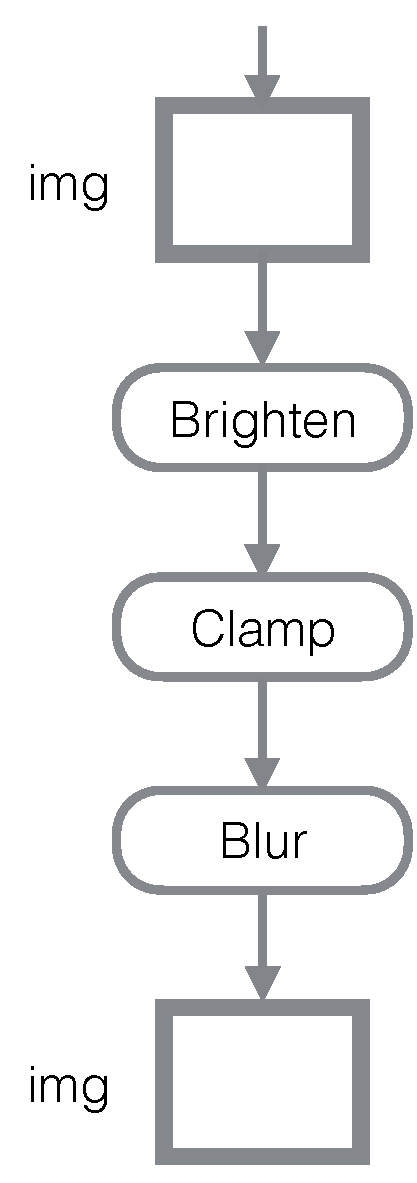
\includegraphics[scale=0.2]{./figures/motivating_example.pdf}

\end{subfigure}
\hspace*{\fill}
\begin{subfigure}{.35\textwidth}
 \begin{lstlisting}[language=C,escapechar=@]
float b1[M][3], b2[M][3], img[N][M][3]
for (i in 0..N)
 for (j in 0..M)
  for (c in 0..3)
   b1[j][c] = 1.5*img[i][j][c]@\label{fig:motivating:code1:stmt1}@
 for (j in 0..M )
  for (c in 0..3)
   b2[j][c] = clamp(b1[i][j][c], 0, 255)@\label{fig:motivating:code1:stmt2}@
 for (j in 0..M)
  for (c in 0..3)
   img[i][j][c] = (b2[j-1][c] + b2[j][c] +@\label{fig:motivating:code1:stmt3}@
                   b2[j+1][c])/3
\end{lstlisting}
\end{subfigure}
\caption{\label{fig:motivating:example} Motivating example.}
\end{figure}


%**********************************************************************************

\begin{figure}[t!]

\centering
\scriptsize

\begin{tabular}{cl}
{\textbf{\normalsize(a)}} &

\begin{lstlisting}[language=C,escapechar=@]
float b1[N][M][3], b2[N][M][3], img[N][M][3]
Parallel for (i in 0..N)
 for (j in 0..M)
  for (c in 0..3)
   b1[i][j][c] = 1.5*img[i][j][c]@\label{fig:motivating:code2:stmt1}@
 for (j in 0..M )
  for (c in 0..3)
   b2[i][j][c] = clamp(b1[i][j][c], 0, 255)@\label{fig:motivating:code2:stmt2}@
 for (j in 0..M)
  for (c in 0..3)
   img[i][j][c] = (b2[i][j-1][c] + b2[i][j][c] +@\label{fig:motivating:code2:stmt3}@
                   b2[i][j+1][c])/3
\end{lstlisting}

\\\hline

{\textbf{\normalsize(b)}} &
\begin{lstlisting}[language=C,escapechar=@]
float b1[N][M][3], b2[N][M][3], img[N][M][3]
Parallel for (i in 0..N)
 for (j in 0..M)
  for (c in 0..3)
   b1[i][j][c] = 1.5*img[i][j][c]@\label{fig:motivating:code3:stmt1}@
   b2[i][j][c] = clamp(b1[i][j][c], 0, 255)@\label{fig:motivating:code3:stmt2}@
 for (j in 0..M)
  for (c in 0..3)
   img[i][j][c] = (b2[i][j-1][c] + b2[i][j][c] +@\label{fig:motivating:code3:stmt3}@
                   b2[i][j+1][c])/3
\end{lstlisting}

\\\hline

{\textbf{\normalsize(c)}} &
\begin{lstlisting}[language=C,escapechar=@]
float b2[N][M][3], img[N][M][3]
Parallel for (i in 0..N)
 for (j in 0..M)
  for (c in 0..3)
   float t = 1.5*img[i][j][c]@\label{fig:motivating:code4:stmt1}@
   b2[i][j][c] = clamp(t, 0, 255)@\label{fig:motivating:code4:stmt2}@
 for (j in 0..M)
  for (c in 0..3)
   img[i][j][c] = (b2[i][j-1][c] + b2[i][j][c] +@\label{fig:motivating:code4:stmt3}@
                   b2[i][j+1][c])/3
\end{lstlisting}

\\\hline

{\textbf{\normalsize(d)}} & 
\begin{lstlisting}[language=C,escapechar=@]
float b2[3][N][M], img[N][M][3]
Parallel for (i in 0..N)
 for (j in 0..M)
  for (c in 0..3)
   float t = 1.5*img[i][j][c]@\label{fig:motivating:code5:stmt1}@
   b2[c][i][j] = clamp(t, 0, 255)@\label{fig:motivating:code5:stmt2}@
 for (j in 0..M)
  for (c in 0..3)
   img[i][j][c] = (b2[c][i][j-1] + b2[c][i][j] +@\label{fig:motivating:code5:stmt3}@
                   b2[c][i][j+1])/3
\end{lstlisting}

\\\hline

{\textbf{\normalsize(e)}} & 
\begin{lstlisting}[language=C,escapechar=@]
float b2[3], img[N][M][3]
Parallel for (i in 0..N)
 for (j in 0..M)
  for (c in 0..3)
   b2[0] = clamp(1.5*img[i][j-1][c], 0, 255)
   b2[1] = clamp(1.5*img[i][j][c], 0, 255)
   b2[2] = clamp(1.5*img[i][j+1][c], 0, 255)
   img[i][j][c] = (b2[0] + b2[1] + b2[2])/3
\end{lstlisting}

\\

\end{tabular}

\caption{
(a) Full expansion of b1 and b2 to allow parallelism;
(b) Loop fusion;
(c) Contraction of b1 and b2 to scalars;
(d) Transformation to AOS (Array Of Structures) for GPU execution; and
(e) Full fusion with redundant computation and contraction}
\label{fig:example-ir}

\end{figure}

In Figure~\ref{fig:motivating:example}, an obvious optimization is the parallelization of the outermost loop (over the \lstinline{i} iterator).  In order to parallelize the loop, we must first expand the two-dimensional arrays \lstinline{b1} and~\lstinline{b2} into three-dimensional arrays.  The resulting code is shown in Figure~\ref{fig:example-ir}-\codeone{}.  Another possible optimization is to fuse the loops of the blur and clamp stages.  The resulting code is shown in Figure~\ref{fig:example-ir}-\codetwo{}

If we further assume that \lstinline{img} is the only consumer of \lstinline{b1} and \lstinline{b2}, then the \lstinline{b1} array can be replaced with a scalar, as shown in Figure~\ref{fig:example-ir}-\codethree{}.  If we plan on executing on a GPU, changing from a Structure-of-Arrays (SoA) memory layout to an Array of Structures (AoS) layout may lead to better performance.  Figure~\ref{fig:example-ir}-\codefour{} shows the code after this transformation.

To maximize parallelism and data locality, we should fuse all loops of the pipeline.  Loop fusion is possible at the expense of redundant computation, as shown in Figure~\ref{fig:example-ir}-\codefive{}.  Since only 3 elements of \lstinline{b2} are computed and then immediately consumed in each iteration of the \lstinline{c} loop, we contract the array \lstinline{b2} into just three elements.

These examples demonstrate that the optimal data layout depends on how the code is scheduled, as well as knowledge about consumers of values produced by the code; that is, the data layout depends on the schedule of the program as well as producer-consumer relationships.
These examples show the need for an intermediate representation that avoids committing to a specific data layout at an early stage, since sometimes it is advantageous to perform data layout mapping only after deciding on the computation schedule and composition.
Trying different schedules and different data mappings for the same schedule also becomes easy with this separation and the search for schedule and data-layout can be automated using an auto-tuner~\cite{opentuner}.
%Furthermore, this separation allow domain specific languages to become fully architecture-independent and portable.

\subsection{Intermediate Representations}
The three intermediate representations of \framework stage the incorporation of algorithm, schedule and data layout into the final program representation.
The IR uses a mathematical representation based on the polyhedral model~\cite{feautrier_dataflow_1991,Karp:1967:OCU:321406.321418,Ancourt:1991:SPL:109625.109631,Bas04,bondhugula_effective_2010} with extensions to support non-quasi-affine\footnote{A detailed definition of quasi-affine constraints is provided in Section~\ref{qaffine}, but in general, quasi-affine expressions are linear expressions over the loop iterators and loop parameters.} iteration spaces~\cite{benabderrahmane_polyhedral_2010,pencil}.  This enables the framework to apply advanced transformations on arbitrary loop nests. A typical workflow for using \framework is illustrated in Figure~\ref{fig:overview}.  DSL compilers parse input programs and perform domain specific optimizations before translating the DSL program into Layer I of the \framework intermediate representation.  The first layer of the IR is then transformed to lower layers (Layer II and Layer III), and finally LLVM IR is generated.

\begin{figure}
 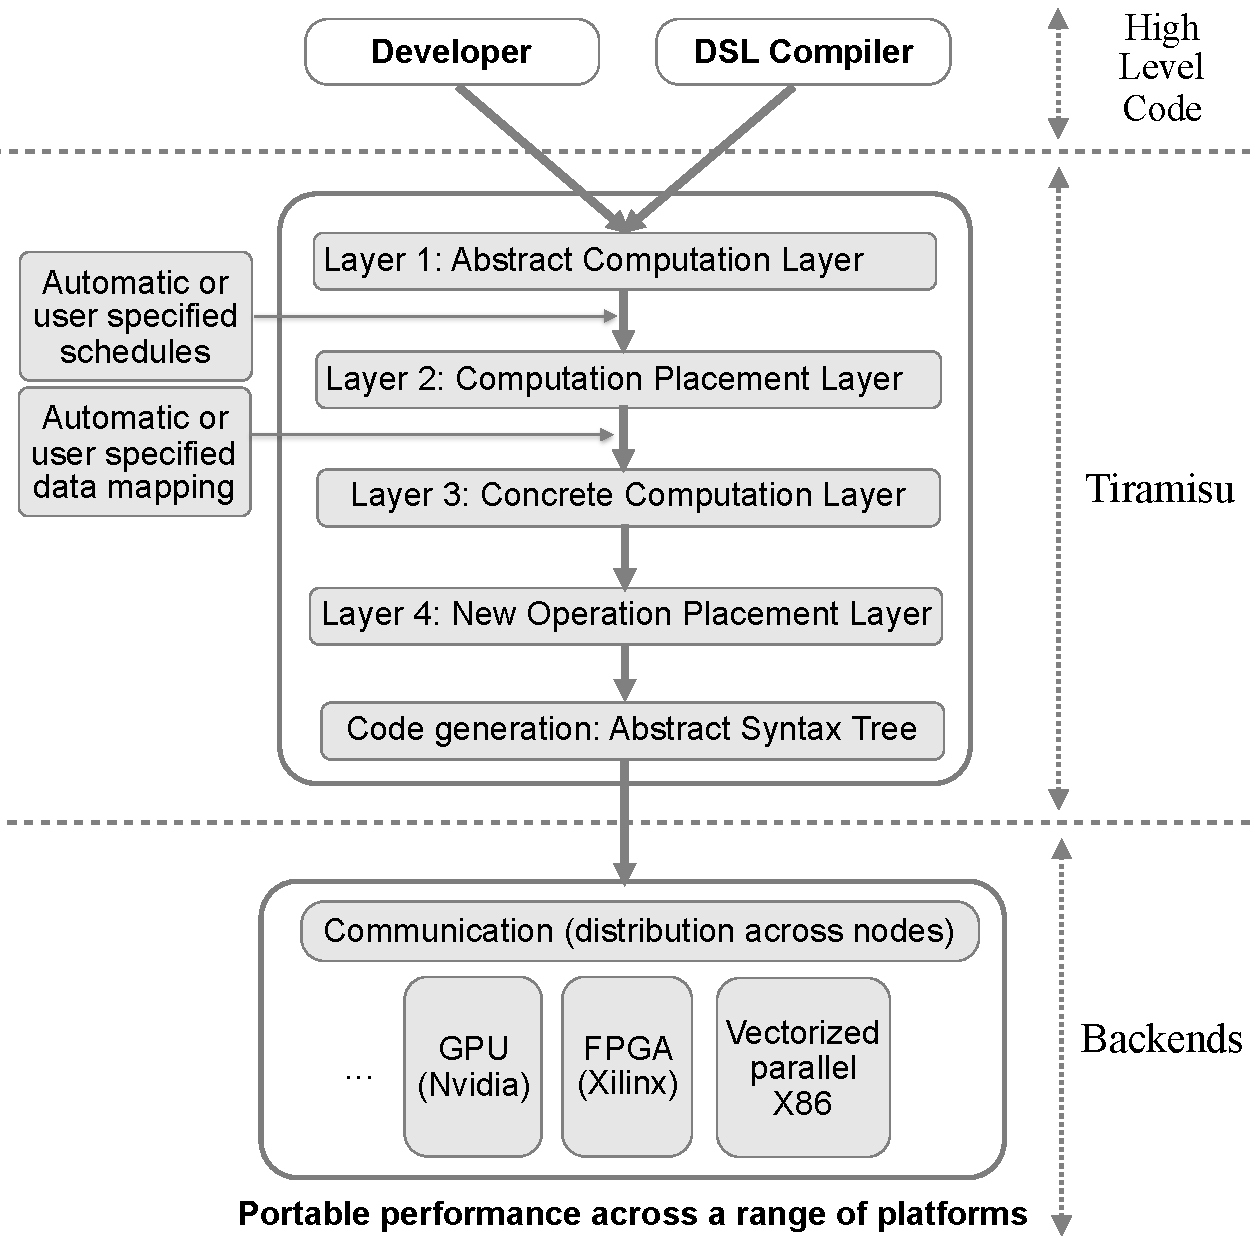
\includegraphics[scale=0.35]{./figures/fista.pdf}
 \caption{\framework overview}
 \label{fig:overview}
\end{figure}

The three layers of the \framework IR are: 
\begin{itemize}
  \item Layer I (\Layerone) specifies the computations (i.e. the algorithm) without specifying the schedule (i.e. when and where the computations occur) or how data should be stored in memory (data layout). As there is no notion of a data location, values are communicated via explicit producer-consumer relationships between the producing statement and all consuming expressions.  
  \item Layer II (\Layertwo) uses a {\it time-\processor vector} to specify when and where the computations occur, i.e. in which order and on which logical processor. This layer does not specify how intermediate values are stored in memory; this simplifies optimization passes at this layer since these passes do not need to perform complicated data-layout transformations. 
  %However, it uses a multi-dimensional time-\processor vector, that can represent many complex computation placements.
  \item Layer III (\Layerthree) makes the data layout concrete, specifying where in memory intermediate values are stored.
\end{itemize}

The separation into levels does not imply that data-layout mapping must always occur after scheduling the computation; in \framework, the user can still specify data layout before scheduling (to constrain the scheduling, for example). However, the separation ensures that the scheduling phase can safely assume no data-layout transformations are required, greatly simplifying scheduling transformations.

%\framework provides mechanisms for transforming the IR into subsequent levels.  Users specify a sequence of transformations to apply (e.g. tiling, splitting, fusion, parallelization, vectorization, or any arbitrary quasi-affine transformation), and the framework applies them and generates code but it does not provide any automatic way to decide which schedules and data layouts are valid, or which will result in the most optimal code. Such automation is beyond the scope of this paper.

While simple primitives and time-processor-vectors provide an easy path from Layer I to Layer III,   
the underlying polyhedral representation  allows the \framework to handle much more complicated iteration spaces and advanced iteration space transformations.
Transformations from iteration space in Layer I to the time-\processor space in Layer II and then the time-\processor vector to the data layout in Layer III can be expressed as quasi-affine relations. %Transformations between layers can also be performed using a non-quasi-affine transformation framework as long as such a framework can start from code in one IR layer and generate another layer of the IR.

\begin{comment}

\begin{figure}
\small

\centering\begin{lstlisting}[language=C,escapechar=@,basicstyle=\linespread{0.9}\small\ttfamily]
for (i in 0..N)
  for (j in 0..M)
    S1
    S2
\end{lstlisting}
(a) Original computation expressed as an imperative program


\begin{tabular}{c|c}
\\\hline
   \begin{tabular}{l@{\hspace{4pt}}r@{\hspace{2pt}}c@{\hspace{2pt}}c@{\hspace{2pt}}c@{\hspace{0pt}}l}
    S1: & [ & $i,$ & $j$, & $0$ & ] \\
    S2: & [ & $i$, & $j$, & 1 & ] \\
    \multicolumn{6}{c}{ (b) Sequential}
   \end{tabular}
     &  
   \begin{tabular}{l@{\hspace{4pt}}r@{\hspace{2pt}}c@{\hspace{2pt}}c@{\hspace{2pt}}c@{\hspace{0pt}}l}
    S1: & [ & $j$, & $i$, & 0 & ] \\
    S2: & [ & $j$, & $i$, & 1 & ] \\
    \multicolumn{6}{c}{ (c) Transposed}
   \end{tabular} \\\hline

    \begin{tabular}{l@{\hspace{4pt}}r@{\hspace{2pt}}c@{\hspace{2pt}}c@{\hspace{2pt}}c@{\hspace{0pt}}l}
    S1: & [ & $i$, & 0, & $j$ & ] \\
    S2: & [ & $i$, & 1, & $j$ & ] \\
    \multicolumn{6}{c}{ (d) Inner loop fission}
   \end{tabular} 
   & 
    \begin{tabular}{l@{\hspace{4pt}}r@{\hspace{2pt}}c@{\hspace{2pt}}c@{\hspace{2pt}}c@{\hspace{0pt}}l}
    S1: & [ & 0, & $i$, & $j$ & ] \\
    S2: & [ & 1, & $i$, & $j$ & ] \\
    \multicolumn{6}{c}{ (e) Outer loop fission}
   \end{tabular} \\\hline
   
    \begin{tabular}{l@{\hspace{4pt}}r@{\hspace{2pt}}c@{\hspace{2pt}}c@{\hspace{2pt}}c@{\hspace{2pt}}c@{\hspace{0pt}}l}
    S1: & [  & $i/N$, & $i\%N$, & $j$, & 0 & ] \\
    S2: & [  & $i/N$, & $i\%N$, & $j$, & 1 & ] \\
    \multicolumn{6}{c}{ (f) Loop split}
   \end{tabular} 
   &
    \begin{tabular}{l@{\hspace{4pt}}r@{\hspace{2pt}}c@{\hspace{2pt}}c@{\hspace{2pt}}c@{\hspace{2pt}}c@{\hspace{0pt}}l}
    S1: & [ & $i/N$, & $j$, & $i\%N$, & 0 & ] \\
    S2: & [ & $i/N$, & $j$, & $i\%N$, & 1 & ] \\
    \multicolumn{6}{c}{ (g) ... \& permuted}
    \end{tabular}  \\\hline
    
    \begin{tabular}{l@{\hspace{4pt}}r@{\hspace{2pt}}c@{\hspace{2pt}}c@{\hspace{2pt}}c@{\hspace{2pt}}c@{\hspace{0pt}}l}
    S1: & [ & $i\%P$ {\it (cpu)}, & $j$, & $i/P$, & 0 & ] \\
    S2: & [ & $i\%P$ {\it (cpu)}, & $j$, & $i/P$, & 1 & ] \\
    \multicolumn{6}{c}{ (h) Outer parallel }
   \end{tabular} 
   &
    \begin{tabular}{l@{\hspace{4pt}}r@{\hspace{2pt}}c@{\hspace{2pt}}c@{\hspace{2pt}}c@{\hspace{2pt}}c@{\hspace{0pt}}l}
    S1: & [ & $i$, & $j/4$, & 0, & $j\%4$ {\it (vec)} & ] \\
    S2: & [ & $i$, & $j/4$, & 1, & $j\%4$ {\it (vec)} & ] \\
    \multicolumn{6}{c}{ (i) Inner vectorized }
   \end{tabular} \\ 

\end{tabular}
 \caption{For a simple loop next with two statements, examples of different time-processor vectors leading to many possible execution arrangements. }
\label{fig:time-processor-vector}
\end{figure}

\end{comment}

%\subsection{Time-Processor Vectors}

% to map an iteration into a \processor and time order.
%The {\it time-\processor vector} in Layer II is a vector indicates the logical time of execution of computations and the processor on which they should be executed.
%Computations in Layer II are represented as {\it time-\processor vectors}.  Each one of those vectors has a name associated to it (the name of the computation). $S1[0,0,0]$, $S2[0,0,1]$, $S1[i,j,0]$ and $S2[i(cpu),j,1]$ are  examples of time-\processor vectors representing computations in Layer II.
%In general, the  time-\processor vector has two types of dimensions: time dimensions and \processor dimensions.
%The time dimensions provide the logical order of execution of the computations while the \processor dimensions indicate on which processor the computations should be executed.
%In the previous example, the first three vectors have time dimensions only, while the last vector has one space dimension.
%We use a tag to indicate that a given dimension is a \processor dimension; this tag indicates mainly the type of processor to which the computations are mapped.%: cpu, gpu, node (for a distributed system), etc.

%Assuming that we have two time-\processor vectors we want to know which vector among the two executes first, then all we need to do is to compare the two vectors lexicographically~\footnote{A \emph{time-\processor vector} $[i_1, \dots, i_k, \dots, i_n]$ lexicographically precedes another time-\processor vector $[i_1', \dots, i_k', \dots, i_n']$ if and only if $\exists k \in \mathbb{N}$ such that $i_1 = i_1' \wedge i_2 = i_2' \wedge \dots \wedge i_k < i_k'$}.
%In the example, $S1[0,0,0]$ precedes $S2[0,0,1]$ lexicographically, so $S1[0,0,0]$ is scheduled to be executed before $S2[0,0,1]$.
%The ability to add dimensions and reorder them freely enables the expression of multiple possible mappings from the original iteration space of the computations to complex execution scenarios.
%Figure~\ref{fig:time-processor-vector} provides examples of different optimizations for a simple algorithm and shows the  time-\processor vectors used to express those optimizations.
%Each of the dimensions of the vector can be an indexed variable, distributing the computation over that dimension or a constant providing a lexical ordering between statements. 
%The algorithms will be using a custom intermediate representation within each DSL, however, we use a classical imperative language representation to describe them in this paper.
%A value can be annotated by a processor type, indicating where that computation will be placed, and indicating that dimension will be run in parallel.





\subsection{Why is an Extended Polyhedral Representation Required}

Example that requires shifting for fusion,

\begin{figure}[ht]

\begin{lstlisting}[language=C,escapechar=@]
/* Loop 1: Ring Blur Filter */
for (i = 1; i < length - 1; i++)
 for (j = 1; i < width - 1; j++)
  Ring[i][j] = (Img[i-1][j-1] + Img[i-1][j] + Img[i-1][j+1]+
                Img[i][j-1] + Img[i][j+1]+
                Img[i+1][j-1]+Img[i+1][j]+ Img[i+1][j+1])/8;

/* Loop 2: Roberts Edge Detection Filter */
for (i = 1; i < length - 2; i++)
 for (j = 2; i < width - 1; j++)
  Img[i][j] = abs(Ring[i][j] - Ring[i+1][j-1])+ abs(Ring[i+1][j] - Ring[i][j-1]);

\end{lstlisting}

\caption{\label{fig:motivating:example2} Second motivating example.}
\end{figure}



\subsection{Three-Layer IR Example}
Figure~\ref{fig:example-ir} shows the code for each one of the optimizations discussed in the previous section along with its three-level IR representation (Layer I, II and III) on the right. A more formal definition of each IR layer and inter-level transformations is presented in Sections~\ref{sec:ir}--\ref{sec:compilation}.  
The Layer I representation, provided by the high-level DSL compiler, is common between all the code variants, regardless of how they are optimized. Porting the code to a new machine does not require changing the algorithm; only the schedule and data mapping need to be changed.
The Layer II representation is the same for code variants that have the same schedule but only differ in the data mapping; this is the case for Figures~\ref{fig:example-ir}-\codetwo{} and~\ref{fig:example-ir}-\codethree{} as scalarization does not require changes to the schedule.

Each line in Layer I of Figure~\ref{fig:example-ir}-\codeone{} (right side in the figure) corresponds to a statement in the original algorithm (left side of the figure): for example, the second line of Layer I represents the line~\ref{fig:motivating:code1:stmt1} in Figure~\ref{fig:example-ir}-\codeone{}.
The first part of that line, which is $\{b_1\ (i, j): 0\leq i < N \wedge 0\leq j < M\}$, represents the iteration space of the statement, while the second part, $a(0)*f_1(i, j)$, is an expression that represents what is computed (note that we represent the scalar $a$ as an array of length 1).
The iteration space is the set of tuples $(i,j)$ such that $0\leq i < N \wedge 0\leq j < M$, and is used to define the set of computations $b_1(i,j)$.  Each computation $b_1(i,j)$ computes the expression $a(0)*f_1(i,j)$.  The set of integer tuples is compactly described by a set of constraints (quasi-affine constraints over the loop iterators and symbolic constants; see Section~\ref{qaffine} for details).  We use $b_1$ as the collective name of the static producer and $b_1(i,j)$ denotes a particular dynamic instance of that producer.  It refers to the value produced by the $(i,j)$ iteration.

%The key idea of this level is to define the computations independent of memory locations and intermediate storage, so this level does not say anything about the order of computations or their storage.  For example, the last line in Figure~\ref{fig:example-ir}, defining the computation of $avg$, is the same regardless of which of the optimized implementations in Figures~\ref{fig:motivating:code1}--\ref{fig:motivating:code4} we represent. 

The computations in Layer I are not ordered.  The order in which they are declared does not have any effect on their actual order of execution.  The actual order of execution is specified in Layer II.
%The order imposed by the producer-consumer relationships is not explicitly represented in the IR layers, but it can be easily computed using polyhedral array data flow analysis~\cite{feautrier_dataflow_1991}. Dependence analysis in Layer I is effective because of the absence of aliasing problems given that the IR does not have any notion of pointers and given that every computation is only defined once.

%For example, whether the computations $out(i,j)$ are stored in a contracted array, in a scalar or whether they are duplicated for execution on different CPUs, the consumer does not need to change.  Only the data mapping (in layer III) needs to be modified depending on the data layout chosen.




An example of the Layer II representation is shown on the right side of Figure~\ref{fig:example-ir}-\codeone{}.
The main difference between Layer I and II is that computations in Layer II are ordered using a time-processor vector while computations in Layer I are not.  The set $\{b_1[1, i (cpu, virtual), 0, j]:  0\leq i < N \wedge 0\leq j < M\}$, in the example, is an ordered set of computations where the time-processor vector $[1, i (cpu, virtual), 0, j]$ orders the computation and maps it to the $i$th virtual CPU.  The tag \emph{(cpu)} for the $i$ dimension indicates that this dimension is a \processor dimension and that each $i$th iteration is mapped to the $i$th CPU. Adding the tag \emph{(virtual)} indicates that the CPU to which the computations are mapped is a virtual CPU; a virtual CPU is mapped by the runtime to any physical CPU during execution.  To identify the logical order of execution between the computations mapped to the same processor, we project out (remove) the \processor{} dimensions and keep only the time dimensions of the time-processor vector ($[1, 0, j]$ in the previous example); then we compare these computations based on their lexicographical order~\footnote{Although the computations have different names, when comparing them we ignore those names and consider that they are all a part of the same time-\processor{} space.}.
%This is denoted as follows $$[i_1, i_2, \dots, i_k, \dots, i_n] \ll [i_1', i_2', \dots, i_k', \dots, i_n']$$.

%Figure~\ref{} shows how we can represent the order of execution of the statements in Figure~\ref{} and their placement using a \emph{time-\processor } vector.

%  A dimension can be a dynamic dimension (usually a loop iterator or a linear combination of the loop iterators and parameters), and can also be a constant (usually used to specify the order between statements that have the same iteration space but only differ in their order within  the statements, . Iteration variables normally provide sequential execution or can be annotated with a virtual processor, providing parallel execution. 

%Although, all the computations in layer II are a part of the same space, which is the time-\processor space, we use different names for the different computations.  Such names in layer II are a syntactic sugar used for convenience only and are ignored when comparing the lexicographical order of computations.

%The transformation of layer I into layer II can be done automatically using an affine schedule (relation) that maps the computations from the iteration space to the time-\processor space.  It can also be done using a non-affine transformation technique as long as the technique guarantees that the generated layer II satisfies some constraints that we specify in Section~\ref{layer2}.

%In the example, Figures~\ref{fig:example-ir}-\codetwo{} and~\ref{fig:example-ir}-\codethree{} share the same Layer II representation.  They only differ in their Layer III representation.

Layer III of Figure~\ref{fig:example-ir}-\codeone{} is the last layer of the \framework IR.  At this layer, we keep the same Layer II representation and add the mapping to data-layout (memory buffers and scalars are also declared in this layer).
This layer indicates where each computation is stored in memory.  In the example, the data mapping $\{b_1[1, i (cpu, virtual), 0, j] \rightarrow {buf}_{b1}[i,j]:  0\leq i < N \wedge 0\leq j < M\}$ indicates that the result of the computation $b_1[1, i (cpu, virtual), 0, j]$ is stored in the array element ${buf}_{b1}[i,j]$.
%(in the contracted array $buf_{b1}[N,3]$).
The data mapping in general is a quasi-affine relation that maps a computation from the time-\processor space to a buffer element (scalars are one element buffers).  \framework allows the expression of all the data-layout mappings that can be expressed as quasi-affine relations (examples provided in Section~\ref{layer3}).
For brevity, the declaration of buffers, their types, their allocation (including when and where they are allocated), are all omitted from the example, but such information must be specified for correct code generation.

Here is another example of data layout mapping: if we want to map the $b_1$ and $b_2$ computations of Figure~\ref{fig:example-ir}-\codefour{} to an array-of-structures, it is sufficient to provide the following mapping to an array $buf_b[N, 2, \boldsymbol{2}]$ where the innermost dimension of the array (in bold) is used to represent a tuple index, which is equivalent to a slot in a structure:

\noindent $\{b_1[1, i (cpu, virtual), j, 0, k] \rightarrow buf_b[i, k, 0]:  0\leq i < N \wedge 0\leq j < M \wedge 0\leq k < 2\}$ \\
$\{b_2[1, i (cpu, virtual), j, 1, k] \rightarrow buf_b[i, k, 1]:  0\leq i < N \wedge 0\leq j < M \wedge 0\leq k< 2\}$ \\

\subsection{Scope of the Intermediate Representation}

The \framework intermediate representation is designed to be used as an IR for DSLs that logically operate over dense data using loop nests and sequences of statements.  In general, this is the case for DSLs in fields such as image processing, dense linear algebra, stencils, etc.
%The schedule and data mappings are either derived automatically or are specified by the user at the DSL language level (as in Halide~\cite{halide_12} for example).
We assume that function calls are inlined and that all iteration spaces are quasi-affine.  %The framework can represent arbitrary iteration spaces (quasi-affine and non-quasi-affine iteration spaces including while loops, loop nests with non-quasi-affine conditionals, loop nests with non-quasi-affine loop bounds, etc.).%  It can automatically transform layer I into layer II if the schedule (transformation relation) is quasi-affine; but allows the user can perform some non-quasi-affine transformations from layer I to layer II.  The framework can represent all types of data-mapping that can be expressed as quasi-affine relations.

In the following section, we provide more details about the formalism that we use to represent integer sets and maps (relations between sets).


\section{Notation and Required Definitions}

In this section, we formally describe the notation and definitions 
used in the rest of the paper.  Readers
familiar with polyhedral libraries such as the Integer Set Library
(ISL)~\cite{verdoolaege_isl:_2010} or Omega~\cite{omega} will be familiar with these
concepts and may skip to the next section.


\paragraph{Presburger formula}

We use an EBNF (Extended Backus-Naur Form) grammar to define Presburger formulas.
\[
\begin{array}{lcl}
\pgrammar{formula} & \gets &  \pgrammar{formula} \wedge \pgrammar{formula} \\ 
        & & ~|~ \pgrammar{formula} \vee   \pgrammar{formula} \\
        & & ~|~ \neg \pgrammar{formula} 
        ~|~ \exists \pgrammar{var}. \pgrammar{formula} \\
        & & ~|~ \forall \pgrammar{var}. \pgrammar{formula}
        ~|~ \pgrammar{atom} \\
                            
\pgrammar{atom} & \gets &  \pgrammar{term} \pgrammar{relop} \pgrammar{term}
                            \\
\pgrammar{term} & \gets &     \pgrammar{numeral}
        ~|~ \pgrammar{term} + \pgrammar{term} \\
        & & ~|~ -\pgrammar{term} \\
        & & ~|~ \pgrammar{numeral} * \pgrammar{term}
        ~|~ \pgrammar{var}
                            \\
\pgrammar{relop} & \gets &    <
        ~|~ \leq
                            ~|~ =
                            ~|~ >
                            ~|~ \geq
                            \\
\pgrammar{var} & \gets &      x
                            ~|~ y
                            ~|~ z
                            ~|~ \dots
                            \\
\pgrammar{numeral} & \gets &  0
                            ~|~ 1
                            ~|~ 2
                            ~|~ \dots
                            \\
\end{array}
\]

Note that $\pgrammar{numeral} * \pgrammar{term}$ is not a general multiplication operator;
it is a shortcut for $\pgrammar{term}+\dots+\pgrammar{term}$.

Presburger arithmetic is used mainly because it is a decidable arithmetic.
That is, there exists an algorithm which decides whether an arbitrary Presburger formula is true (valid) or not, which is important for many polyhedral operations.


\paragraph{Quasi-Affine Constraints}
\label{qaffine}

A \emph{quasi-affine constraint} is a constraint over integer values and integer variables involving only the operators \lstinline{+}, \lstinline{-}, $\times$, \lstinline{/}, \lstinline{mod}, \lstinline{&&}, \lstinline{||}, \lstinline{<}, \lstinline{<=}, \lstinline{>}, \lstinline{>=}, \lstinline{==}, \lstinline{!=}, and the ternary \lstinline{?:} operator, where the second argument of \lstinline{/} and \lstinline{mod} must be a (positive) integer literal, and where at
least one of the arguments of $\times$
must be a constant expression.
An example of a quasi-affine constraint for a statement in a loop nest is $10\times i+j+n>0$, where $i$ and $j$ are loop iterators and $n$ is a
\emph{symbolic constant} (i.e., a variable that has an unknown but fixed value for the duration of
an execution).  An example of a non-quasi-affine constraint is $i \times i>0$, because we require one of the arguments be a constant.

\paragraph{Integer Sets}

An \emph{integer set} is a set of integer tuples from $\mathbb{Z}^d$ that can be specified using  quasi-affine constraints. $d$ is the dimensionality of the set (the number of integers in each tuple) and a d-tuple is represented as $[a_1, a_2, \dots, a_d]$.  An example of a set of integer tuples is:
$$\{[1,1]; [2,1]; [3,1]; [1,2]; [2,2]; [3,2]\}$$

Instead of listing all the integer tuples of the set, we describe the set using quasi-affine constraints:
$$\{S[i,j]:  1 \leq i \leq 3 \wedge 1 \leq j \leq 2\}$$

\noindent where $i$ and $j$ are the dimensions of the set.
The tuples of a set can optionally have a common name, such as
$S$ in this example.

In general, an integer set has the form
$$S = \{N[\vec{s}] | f(\vec{s}, \vec{p})\}$$

\noindent with $\vec{s}$ representing the integer tuples of
the integer set ($\vec{s} \in \mathbb{Z}^d$), $N$, a common name
for all the tuples $\vec{s}$ usually used as the name of computations, $d$ the dimensionality of the set, $\vec{p} \in \mathbb{Z}^e$ a vector of $e$ parameters and $f(\vec{s}, \vec{p})$ a Presburger formula that evaluates to true, if and only if $\vec{s}$ is an element of $S$ for the given parameters $\vec{p}$.

\subsection{Maps}

A map is a relation between two integer sets.  For example
$$M = \{S1[i,j] \rightarrow S1[i+2,j+2] : 1 \leq i \leq 3 \wedge 1 \leq j \leq 2\}$$

\noindent represents a relation between two sets. The first set
is called the \emph{domain} or the \emph{source}
and the second is called the \emph{range} or the
\emph{sink}.
Figure~\ref{fig:map} shows a graphical representation of
the map $M$.

\begin{figure}[th]
  \centering
  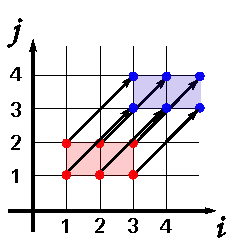
\includegraphics[scale=0.7]{figures/map.pdf}
  \caption{Graphical representation of a map}
  \label{fig:map}
\end{figure}

In general, a map has the form
$$M = \{A[\vec{s}] \rightarrow B[\vec{o}], (\vec{s}, \vec{o}) \in \mathbb{Z}^{d_1}\times\mathbb{Z}^{d_2} | f(\vec{s}, \vec{o}, \vec{p})\}$$

\noindent where $A[\vec{s}]$ represents the domain or the
source and $B[\vec{o}]$ represents the range or the sink.
$d_1$ and $d_2$ are the dimensionalities of $\vec{s}$
and $\vec{o}$, $\vec{p} \in \mathbb{Z}^e$ is a vector of $e$ parameters and $f(\vec{s}, \vec{o}, \vec{p})$ is a Presburger formula that evaluates to true if and only if there is a relation from $\vec{s}$ to $\vec{o}$ in $M$ for the given parameters
$\vec{p}$.


\section{\label{sec:ir}The \framework{} IR}

%\subsection{Example}

%% Challenge of scheduling
%Figures~\ref{fig:example-ir}-\codetwo{} (Schedule) and ~\ref{fig:example-ir}-\codethree{} (Schedule) show how a simple collection of scheduling commands can map the architecture independent program into different architectural configurations. 

%% The MPI+OpenMP+CUDA Challenge
%Figure~\ref{fig:example-ir}-\codethree{} (left) shows an example where the algorithm is mapped to a GPU cluster using simple scheduling commands and without the need to change the algorithm or to write code in different languages and libraries.


\begin{figure*}[t!]
    \centering
    \scriptsize
    \setlength\tabcolsep{4pt}
\begin{tabular}{cl|@{}l}
\multicolumn{3}{c}{\textbf{Constraints:} \boldsymbol{$\ \ \ C_n: 0\leq i < N, \ \ \ \ \ \ C_m: 0\leq j < M, \ \ \ \ C_{m'}: 1\leq j < M-1, \ \ \ \ C_{k}: 0\leq c < 3, \ \ \ \ C_{q}: 0\leq q < NUM\_NODES$}}
\\\hline
  &
    \ \ \ \ \ \ \ \ \ \ \ \ \ \ \ \ \ \ \ \ \ \ \ 
    \textbf{Different Code Optimizations}
  &
    \ \ \ \ \ \ \ \ \ \ \ \ \ \  
    \textbf{\framework representation (Layer I, Layer II and Layer III)}
\\\hline

{\textbf{\normalsize(a)}} &
\begin{lstlisting}[language=C,escapechar=@]
// Original unoptimized code
for (i in 0..N)
  for (j in 0..M)
    for (c in 0..3)
      b1[j][c] = 1.5*img[i][j][c] // brightening @\label{fig:motivating:code1:stmt1}@
  for (j in 0..M )
    for (c in 0..2)
      b2[j][c] = clamp(b1[j][c], 0, 255)@\label{fig:motivating:code1:stmt2}@
  for (j in 1..M-1)
    for (c in 0..3)
      out[i][j][c] = (b2[j-1][c] + b2[j][c] + @\label{fig:motivating:code1:stmt3}@
                      b2[j+1][c])/3
\end{lstlisting}
    &  
\begin{tabular}{c|l}
\multirow{12}{1cm}{\textbf{Layer I}}
    & \\
    & \\
    & \\
    & \\
    & The constraints $C_n$, $C_m$ and $C_k$ are defined above.\\
    & {\color{listingmauve}{$\{b_1\ (i, j, c): C_n \wedge C_m \wedge C_k\} $}} \ \ \ :\ \ \ $1.5*img(i, j, c)$\\
    & {\color{listingmauve}{$\{b_2\ (i, j, c): C_n \wedge C_m  \wedge C_k\}$}} \ \ \ :\ \ \ $\ clamp(b_1(i, j, c), 0, 255)$ \\
    & {\color{listingmauve}{$\{out(i, j, c): C_n \wedge C_{m'} \wedge C_k\}$}} \ :\  \ \ $(b_2(i,j-1,c)+b_2(i,j,c)+b_2(i,j+1,c))/3$\\
    & \\
    & \\
    & \\
    & \\
\end{tabular}
    \\\hline
{\textbf{\normalsize(b)}} &
\begin{lstlisting}[language=C,escapechar=@]
// Code optimized for CPU
@{\color{listingkeywordcolor}{\textbf{parallel}}}@ for (i in 0..N)
  for (j in 0..M)
    for (c in 0..3)
      float t = 1.5*img[i][j][c]@\label{fig:motivating:code2:stmt1}@
      b2[i][j][c] = clamp(t, 0, 255)@\label{fig:motivating:code2:stmt2}@
  for (j in 1..M-1)
    for (c in 0..3)
      out[i][j][c] = (b2[i][j-1][c] + 
                      b2[i][j][c] +@\label{fig:motivating:code2:stmt3}@
                      b2[i][j+1][c])/3
\end{lstlisting}
    & 
\begin{tabular}{c|l}
 \multirow{3}{*}{\textbf{Schedule}}
 & $b_2$.after($b_1$, c)\\
 & $b_1$.parallel(i); \ \ $b_2$.parallel(i); \ \  $out$.parallel(i)\\
 & $b_1$.store\_in($t$); \ \ $b_2$.store\_in($buf_{b2}[i, j , c]$); \ \  $out$.store\_in($buf_{out}[i, j , c]$);\\
 \hline
 \multirow{6}{*}{\textbf{Layer II}}
    & {\color{listinggreen}{// Layer II generated from Layer I using the schedule}}\\
    & \\
    & {\color{listingmauve}{$\{\ b_1(i (cpu), 0, j, c, 0) : C_n \wedge C_m \wedge C_k\}$}}: $1.5*img(i, j, c)$\\
    & {\color{listingmauve}{$\{\ b_2(i (cpu), 0, j, c, 1): C_n \wedge C_m \wedge C_k\}$}} : $clamp(b_1(i, 0, j, c, 0), 0, 255)$\\
    & {\color{listingmauve}{$\{out(i (cpu), 1, j, c, 0): C_n\wedge C_{m'} \wedge C_k \}$}}:\\
    &$  (b_2(i,0,j-1,c,1)+b_2(i,0,j,c,1)+b_2(i,0,j+1,c,1))/3$\\\hline
 \multirow{5}{*}{\textbf{Layer III}}
    & {\color{listinggreen}{Layer III = Layer II representation + the following data \ mapping}}\\
    & \\
    & $\{b_1\ (i (cpu), 0, j, c, 0) \rightarrow t: C_n \wedge C_m \wedge C_k\}$\\
    & $\{b_2\ (i (cpu), 0, j, c, 1) \rightarrow buf_{b2}[i,j,c]: C_n \wedge C_m \wedge C_k\}$\\
    & $\{out(i (cpu), 1, j, c, 0) \rightarrow buf_{out}[i,j,c]: C_n \wedge C_{m'} \wedge C_k\}$\\\hline
\end{tabular}  
    \\\hline
    {\textbf{\normalsize(c)}} &
\begin{lstlisting}[language=C,escapechar=@]
// Code optimized for multi-GPU
@{\color{listingkeywordcolor}{\textbf{distributed}}}@ for (q in 0..NUM_NODES)
  @{\color{listingkeywordcolor}{\textbf{gpu}}}@ for (i in 0..N/NUM_NODES)
    @{\color{listingkeywordcolor}{\textbf{gpu}}}@ for (j in 0..M)
     for (c in 0..3)
       float t = 1.5*img[i][j][c]@\label{fig:motivating:code2:stmt1}@
       b2[c][i][j] = clamp(t, 0, 255)@\label{fig:motivating:code2:stmt2}@
@{\color{listingkeywordcolor}{\textbf{distributed}}}@ for (q in 0..NUM_NODES)       
  @{\color{listingkeywordcolor}{\textbf{gpu}}}@ for (i in 0..N/NUM_NODES)
    @{\color{listingkeywordcolor}{\textbf{gpu}}}@ for (j in 1..M-1)
      for (c in 0..3)
        out[i][j][c] = (b2[c][i][j-1] +
                        b2[c][i][j] +@\label{fig:motivating:code2:stmt3}@
                        b2[c][i][j+1])/3
\end{lstlisting}
    & 
\begin{tabular}{c|l}
 \multirow{6}{*}{\textbf{Schedule}}
 & $b_2$.after($b_1$, c);   $out$.after($b_2$, root);\\
 & $b_1$.split(i, N/NUM\_NODES, q, i);   $b_2$.split(i, N/NUM\_NODES, q, i); \\ 
 & $out$.split(i, N/NUM\_NODES, q, i); \\
 & $b_1$.store\_in($t$); \ \ $b_2$.store\_in($buf_{b2}[c, i, j]$); \ \  $out$.store\_in($buf_{out}[i, j, c]$);\\
 & $b_1$.gpu(i,j); \ \ $b_2$.gpu(i,j); \ \  $out$.gpu(i,j)\\
 & $b_1$.distribute(q); $b_2$.distribute(q); $out$.distribute(q); \\
 \hline
 \multirow{7}{*}{\textbf{Layer II}}
    & {\color{listinggreen}{// Layer II generated from Layer I using the following schedule}}\\
    & \\
    & {\color{listingmauve}{$\{\ b_1(0, q(node), i(gpu), j(gpu), c, 0) : C_q \wedge C_n \wedge C_m \wedge C_k\}$}}: $1.5*img(i, j, c)$\\
    & {\color{listingmauve}{$\{\ b_2(0, q(node), i(gpu), j(gpu), c, 1): C_q \wedge C_n \wedge C_m \wedge C_k\}$}} : \\
    & $clamp(b_1(0, q, i, j, c, 0), 0, 255)$\\
    & {\color{listingmauve}{$\{out(1, q(node), i(gpu), j(gpu), c, 0): C_q \wedge C_n\wedge C_{m'} \wedge C_k \}$}}:\\
    &$  (b_2(0,q,i,j-1,c,0)+b_2(0,q,i,j,c,1)+b_2(1,q,i,j+1,c,0))/3$\\\hline
 \multirow{5}{*}{\textbf{Layer III}}
    & {\color{listinggreen}{// Same as Layer III in (b) except the mapping of $b_1$ and $b_2$ should be replaced}} \\
    & {\color{listinggreen}{with the following}} \\
    & \\
    & $\{b_1\ (0, q(node), i(gpu), j(gpu), c, 0) \rightarrow t: C_q \wedge C_n \wedge C_m \wedge C_k\}$\\
    & $\{b_2\ (0, q(node), i(gpu), j(gpu), c, 1) \rightarrow buf_{b2}[c,i,j]:  C_q \wedge C_n \wedge C_m \wedge C_k\}$\\
\end{tabular}
    \\\hline
    \end{tabular}
    \caption{Three versions of the motivating example (left) and their equivalent Layer I, II and III representations (right)}
    \label{fig:example-ir}
    \vspace{-0.25cm}
\end{figure*}


In the following section, we provide more details about the four layers of \framework.

\begin{table}
    \scriptsize
    \setlength\tabcolsep{1pt}
    \begin{tabular}{l|l}
        \hline
        \multicolumn{2}{c}{\textbf{Commands to transform Layer I into Layer II}} \\
        \multicolumn{2}{c}{We assume that C and P are computations} \\\hline
        \textbf{Command} & \textbf{Description} \\\hline
        \texttt{C.interchange(i, j)} & Interchange the dimensions of C (loop interchange) \\\hline
        \texttt{C.shift(i, s)} & Loop shifting (shift the dimension i by s iterations) \\ \hline
        \texttt{C.split(i, s, i0, i1)} & Split the dimension i by s. (i0, i1) are the new dimensions\\ \hline
        \begin{tabular}{ll} \texttt{C.tile(}& \texttt{i,j,t1,t2,}\\ & \texttt{i0,j0,i1,j1)}
        \end{tabular} & 
        \begin{tabular}{l}
        Tile the dimensions (i,j) of the computation C by $t1\times t2$.\\
        The names of the new dimensions are (i0, j0, i1, j1).\end{tabular}\\ \hline
        \texttt{P.compute}\_at(C, j) & Compute the computation \emph{P} in the loop nest of \emph{C} at loop\\
        & level j.  This might introduce redundant computations.\\
        \hline
        \texttt{C.vectorize(i, v)} & Vectorize the dimension i by a vector size v\\\hline
        \texttt{C.unroll(i, v)} & Unroll the dimension i by a factor v\\\hline
        \texttt{C.parallelize(i)} & Mark the dimension i as a space dimension (cpu)\\\hline
        \texttt{C.distribute(i)} & Mark the dimension i as a space dimension (node)\\\hline
        \texttt{C.after(B, i)} & Indicate that C should be ordered after B at the loop level i\\
        &(they have the same order in all the loop levels above i)\\
        \hline
        \texttt{C.inline()} & Inline C in all of its consumers\\ \hline
        \texttt{C.set\_schedule()} & Set the schedule of C, i.e.,a map that transforms Layer I to \\ & Layer II\\\hline
        \texttt{C.gpu(i0,i1,i2)} & Mark the dimensions i0, i1 and i2 to be executed on the GPU \\\hline
        \texttt{C.fpga()} & Generate HLS code for the computation C\\\hline
        \texttt{C.pipeline(i)} & Mark the dimension i to be pipelined (FPGA)\\\hline
        \multicolumn{2}{c}{} \\
        \multicolumn{2}{c}{\textbf{Commands to add data mapping to Layer III}} \\\hline
        \texttt{Buffer b(...)} & Declare a buffer b (size, type, ...) \\\hline
        \texttt{C.set\_access()} & Set the access relation for the computation C
        \\\hline
        \texttt{C.store\_in(buff[i0,..])} & Store the result of the computation $C(i0, ...)$ in buff[i0, ...]
        \\\hline
        \texttt{C.auto\_allocate\_map()} & Allocate a buffer for C and map C to it\\ \hline
        \texttt{C.set\_access()} & Map C to a buffer access\\ \hline
        \texttt{C.storage\_fold(i, d)} & Contract the dimension i of the buffer associated to C to \\
        & make its size d \\\hline
        \texttt{create\_transfer(...)} & Create a pair of send \& receive communication statements \\
        \hline
        \texttt{C.partition(b, type)} & Mark the buffer b to be partitioned in a complete, cyclic or \\ & block way (FPGA)\\\hline
    \end{tabular}
    \caption{Examples of \framework{} Scheduling Commands}
    \label{tab:scheduling}
    \vspace{-0.5cm}
\end{table}




The input to \framework{} is the Layer I computations and a set of scheduling and data layout commands.  Layer II is generated by applying the schedule to Layer I.
Commands for buffer allocation, data layout mapping, and communication (among CPU nodes for example) are then added to the Layer II representation; this result constitutes Layer III. An annotated abstract syntax tree (AST) is then generated from Layer III.  This AST is traversed to generate the target code.

In this section, we describe in detail the three representations used in \framework{}.  We also describe scheduling via  high-level scheduling commands as well as low level scheduling maps. We begin by showing an example.


\vspace{-0.25cm}
\subsection{An Example in the Four-Layer IR}

We first provide an overview of the concepts of polyhedral sets and maps.  More details and a formal definition of these concepts are provided in the Appendix.

An \emph{integer set} is a set of integer tuples described using affine constraints.  An example of a set of integer tuples is $\{(1,1); (2,1); (3,1); (1,2); (2,2); (3,2)\}$.
Instead of listing all tuples in a set, we describe the set using affine constraints over loop iterators and symbolic constants: $\{S(i,j): 1 \leq i \leq 3 \wedge 1 \leq j \leq 2\}$ where $i$ and $j$ are the dimensions of the set.

A map is a relation between two integer sets.  For example $\{S1(i,j) \rightarrow S2(i+2,j+2) : 1 \leq i \leq 3 \wedge 1 \leq j \leq 2\}$ is a map between tuples in the set S1 and tuples in the set S2 (e.g. the tuple $S1(i,j)$ maps to tuple $S2(i+2,j+2)$).  We use the Integer Set Library (ISL)~\cite{verdoolaege_isl:_2010} notation for sets and maps.

Figure~\ref{fig:example-ir} shows the code for each optimized implementation discussed in the previous section.
%along with its three-level IR
%representation (Layer I, II and III) on the right.
%A more formal definition of each IR layer and inter-level transformations is presented in Section~\ref{sec:ir}.  
The original, unoptimized code is shown in Figure~\ref{fig:example-ir}-\codeone{}, with the right side showing the Layer I representation.
This Layer I representation is the same for all the code variants, as this layer specifies the computation in a high-level form separate from scheduling.   %Porting the code to a new machine does not require changing the algorithm; only the schedule and data mapping need to be changed.

Each line in Layer I of Figure~\ref{fig:example-ir}-\codeone{} (right side in the figure) corresponds to a statement in the algorithm (left side of the figure): for example, the first line of Layer I represents the line~\ref{fig:motivating:code1:stmt1} in Figure~\ref{fig:example-ir}-\codeone{}.
The first part of that line\footnote{The constraints $C_n$, $C_m$, and $C_k$ have been expanded inline}, which is

\begin{lstlisting}[language=C,escapechar=@,numbers=none]
        {@$b_1$@(i,j,c): 0<=i<N and 0<=j<M and 0<=c<3}
\end{lstlisting}

\noindent specifies the iteration domain of the statement, while the second part, $1.5*img(i, j, c)$, is the computed expression.
%Each computation $b_1(i,j,c)$ calculates the expression $1.5*img(i,j,c)$.
The iteration domain is the set of tuples $b_1(i,j,c)$ such that $0\leq i < N \wedge 0\leq j < M \wedge 0\leq c < 3$.
%The set of integer tuples is compactly described by a set of constraints (affine constraints over the loop iterators and symbolic constants).  We use $b_1$ as the collective name of the static producer and $b_1(i,j,c)$ denotes a particular dynamic instance of that producer, referring to the value produced by the $(i,j,c)$ iteration.
Computations in Layer I are not ordered.  The declaration order does not affect their order of execution, which is specified in Layer II.  
%The key idea of this level is to define the computations independent of memory locations and intermediate storage, so this level does not say anything about the order of computations or their storage.  For example, the last line in Figure~\ref{fig:example-ir}, defining the computation of $avg$, is the same regardless of which of the optimized implementations in Figures~\ref{fig:motivating:code1}--\ref{fig:motivating:code4} we represent. 


%The order imposed by the producer-consumer relationships is not explicitly represented in the IR layers, but it can be easily computed using polyhedral array data flow analysis~\cite{feautrier_dataflow_1991}. Dependence analysis in Layer I is effective because of the absence of aliasing problems given that the IR does not have any notion of pointers and given that every computation is only defined once.

%For example, whether the computations $out(i,j)$ are stored in a contracted array, in a scalar or whether they are duplicated for execution on different CPUs, the consumer does not need to change.  Only the data mapping (in layer III) needs to be modified depending on the data layout chosen.


Figure~\ref{fig:example-ir}-\codetwo{} shows the first optimized version of the code.  The schedule on the right side is the set of scheduling and data layout commands that produce this version of the code.  The scheduling commands are presented in Table~\ref{tab:scheduling}.  Layer II is generated automatically by applying these commands to Layer I.
\framework provides a large set of high-level scheduling and data layout transformation commands. % (38 high level and low level commands). Table~\ref{tab:scheduling} shows examples of these commands.
The Layer II representation is also shown in Figure~\ref{fig:example-ir}-\codetwo{}.
Computations in Layer II are ordered based on their lexicographical order\footnote{For example the computation $S0(0, 0, 0)$ is lexicographically before the computation \mbox{$S0(0, 0, 1)$} and the computations $S0(0, i, 0)$ are lexicographically before the computations $S0(1, i, 0)$}.  The set

\begin{lstlisting}[language=C,escapechar=@,numbers=none]
{@$b_1$@(i (cpu), 0, j, c, 0):  0<=i<N and 0<=j<M and 0<=c<3}
\end{lstlisting}

\noindent in the example, is an ordered set of computations.
%Each computation $b_1(i (cpu), 0, j, c, 0)$ is mapped for execution on the $i$th CPU.  
The tag \emph{(cpu)} for the $i$ dimension indicates that this dimension is a \processor dimension and that each $i$-th iteration is mapped to the $i$-th CPU.  In Layer II, the computation order is controlled by a total ordering of these tuples.
%Adding the tag \emph{(virtual)} to the \emph{(cpu)} tag would indicate that the CPU to which the computations are mapped is a virtual CPU that will be mapped by the runtime to any physical CPU during execution.

%Layer II is usually generated automatically from Layer I using scheduling commands.  A scheduling commands in \framework gets translated to an affine relation (function) that transforms the iteration domain.  This affine relation also modifies the accesses automatically as necessary.

%To identify the logical order of execution between the computations mapped to the same processor, we project out (remove) the \processor{} dimensions and keep only the time dimensions of the time-processor vector ($[1, 0, j]$ in the previous example); then 
%The order of execution of computation is defined by their lexicographical order~\footnote{Although the computations have different names, when comparing them we ignore those names and consider that they are all a part of the same time-\processor{} space.}.
%This is denoted as follows $$[i_1, i_2, \dots, i_k, \dots, i_n] \ll [i_1', i_2', \dots, i_k', \dots, i_n']$$.

%Figure~\ref{} shows how we can represent the order of execution of the statements in Figure~\ref{} and their placement using a \emph{time-\processor } vector.

%  A dimension can be a dynamic dimension (usually a loop iterator or a linear combination of the loop iterators and parameters), and can also be a constant (usually used to specify the order between statements that have the same iteration space but only differ in their order within  the statements, . Iteration variables normally provide sequential execution or can be annotated with a virtual processor, providing parallel execution. 

%Although, all the computations in layer II are a part of the same space, which is the time-\processor space, we use different names for the different computations.  Such names in layer II are a syntactic sugar used for convenience only and are ignored when comparing the lexicographical order of computations.

%The transformation of layer I into layer II can be done automatically using an affine schedule (relation) that maps the computations from the iteration space to the time-\processor space.  It can also be done using a non-affine transformation technique as long as the technique guarantees that the generated layer II satisfies some constraints that we specify in Section~\ref{layer2}.

%In the example, Figures~\ref{fig:example-ir}-\codetwo{} and~\ref{fig:example-ir}-\codethree{} share the same Layer II representation.  They only differ in their Layer III representation.

Layer III in Figure~\ref{fig:example-ir}-\codetwo{}  adds data layout mapping to Layer II, concretizing where each computation is stored (memory buffers and scalars are also declared in this layer).
%This layer indicates where each computation is stored in memory.  
In the example, the data mapping

\begin{lstlisting}[language=C,escapechar=@,numbers=none]
{@$b_2$@(0,i(cpu),j,c,1) @$\rightarrow {buf}_{b2}$@[i,j,c]:
    0<=i<N and 0<=j<M and 0<=c<3}
\end{lstlisting}

indicates that the result of the computation $b_2(0, i (cpu), j, c,1)$ is stored in the array element ${buf}_{b2}[i,j,c]$.
%(in the contracted array $buf_{b1}[N,3]$).
Data mapping in \framework is an affine relation that maps a computation from Layer II to a buffer element; scalars are single-element buffers.  \framework allows the expression of any data-layout mapping that can be expressed as an affine relation (examples provided in Section~\ref{layer3}).
For brevity, the declaration of buffers, their types, their allocation (including when and where they are allocated), are all omitted from the example, but such information must be specified for correct code generation.

%Here is another example of data layout mapping: if we want to map the $b_2$ computation to a structure-of-arrays as in Figure~\ref{fig:example-ir}-\codefour{}, it is sufficient to provide the following mapping $\{b_2[1, i (cpu), j, c] \rightarrow {buf}_{b2}[\boldsymbol{c},i,j]:  0\leq i < N \wedge 0\leq j < M \wedge 0\leq c < 3\}$ where the outermost dimension of the array (in bold) is used to represent a tuple index, which is equivalent to a slot in a structure.

%The other codes Figure~\ref{fig:example-ir} shows the three layers that correspond to the code in Figure~\ref{fig:example-ir}-\codefive{}.  Layer I in this figure is identical to Layer I in Figure~\ref{fig:example-3ir-1}.  Layer II expresses three transformations: redundant computations, fusion of loops and shifting.  This layer can be generated automatically using 3 simple high level scheduling commands.  In Layer III, first, we perform array contraction (storage folding) and we map the output computation to the input buffer (\lstinline{img}) to perform inplace computations.




\vspace{-0.25cm}
%\subsection{The Three-Layers of \framework{}}

\subsection{Layer I: \Layerone}
\label{layer1}

The first layer defines abstract computations, which are not yet scheduled or mapped to memory.
%This layer is defined as a set of iteration domains where each iteration domain is composed of a set of computations.
Each \textit{computation} represents an expression that should be computed.  % that performs operations within a loop, containing other computations and literal constants. A formal definition is provided in Appendix~\ref{appendixlayers}.
%Non-loop statements have an iteration domain of a single point.

As an example, the following code

\begin{lstlisting}[language=C,escapechar=@]
for (i in 0..4)
 for (j in 0..4)
   if (i < j && i != 2)
     A[i][j] = cos(i);
\end{lstlisting}

\noindent can be represented in Layer I as

\begin{lstlisting}[language=C,escapechar=@,numbers=none]
{A(i,j): 0<=i<4 and 0<=j<4 and i<j and i!= 2}: cos(i)
\end{lstlisting}

\noindent though it is important to remember that this representation, unlike the pseudocode above, does not necessarily store results to memory locations.
$A(i,j)$ is the computation, while the constraints over $i$ and $j$ define the iteration domain.  The second part, $cos(i)$, is the computed expression.

Computations in Layer I are in Static Single Assignment (SSA) form~\cite{Cytron:1991:ECS:115372.115320}; each computation is defined only once (we use the $\phi$ operator to deal with branches as in classical SSA).

\paragraph{Reductions and Updates}

Reductions and updates do not fit naturally in the memory-independent model used within \framework{}, and thus we treat them as a special case.  To implement algorithms that perform a reduction or update a variable (a histogram for example), we declare a new computation for each update.  These computations will all be mapped to the same buffer in Layer III.
% these computations to the same buffer.
%expand the iteration domain and add a new dimension for versioning.
For example, a dense matrix multiplication, which has a reduction, is represented in Layer I as follows:

\begin{lstlisting}[language=C,escapechar=@,numbers=none]
{c0(i,j):  0<=i<N and 0<=j<N}: 0
{c1(i,j,k): 0<=i<N and 0<=j<N and 1<=k<N}:
    @$\phi($@c0(i,j), c1(i,j,k-1)) + A(i,k) * B(k,j)
\end{lstlisting}

% When generating the third layer for the matrix multiplication code, each computation $c(i,j,k)$ should be mapped to the buffer \lstinline{bufc[i,j]}.  This will produce a reduction.
%When generating Layer III IR from this code, the computations \lstinline{c0(i,j)} and \lstinline{c1(i,j,k)} will be mapped to the same 2-dimensional buffer, producing an update and a reduction.

Since $c1(i,j,k)$ needs to read the results of the computations $c0(i,j)$ and $c1(i,j,k-1)$, we use the $\phi$ node to merge them into one expression $\phi(c0(i,j), c1(i,j,k-1))$ (although the use of $\phi$ nodes in this case can be avoided, in the general case the use of $\phi$ nodes is necessary to support  cases such as the definition of computations within data-dependent conditions).

%$\{c[i,j,k] \rightarrow buf_c[i,j]:  0\leq i < N \wedge 0\leq j < N \wedge 0 \leq k < N \}$

% Since in the Layer I of \framework{} the data layout is not specified and since \framework{} computations can only read values produced by other computations but not directly read arrays from memory, the following natural question arises: how does \framework{} handle input arrays (program inputs).  The solution to this is to wrap any input buffer into a computation.  That is, represent the buffer as a computation in Layer I.  

%\paragraph{Input Arrays}

%The data layout of input arrays also do not fit naturally. Because Layer I does not specify data layout, program inputs are wrapped by a computation in Layer I.  As a result, the rest of the program is made memory-independent.

%Because Layer I does not specify data layout, program inputs are wrapped by a computation in Layer I.
%As a result, the rest of the program is made memory-independent.  For example, in Figure~\ref{fig:example-ir}-\codeone{}, if the input image \lstinline{img} was not computed in previous stages of the pipeline but was instead passed as an input buffer to the program, it would require a wrapper computation.  Only the computation \lstinline{b1} changes:

%\begin{lstlisting}[language=C,escapechar=@,numbers=none]
%{wrapper_img(i,j,c): 0<=i<N and 0<=j<M and 0<=c<3}: ()
%{b1(i,j,c): 0<=i<N and 0<=j<M and 0<=c<3}:
%    1.5*wrapper_img(i, j, c)
%\end{lstlisting}

%The other computations do not change.  The appropriate data mapping would be added in Layer III to map the wrapper computation \lstinline{wrapper_img} to the \lstinline{img} buffer.  In the example, the Layer III data mapping of the computation \lstinline{wrapper_img} would be modified as follows:

%\begin{lstlisting}[language=C,escapechar=@,numbers=none]
%{wrapper_img(i,j,c) -> img[i,j,c]:
%    0<=i<N and 0<=j<M and 0<=c<3}
%\end{lstlisting}


% The following data mapping should have been added in the third layer

% $\{wrapper1(i,j) \rightarrow buf1[i,j]:  0\leq i < N \wedge 0\leq j < N \}$

% $\{wrapper2(i,j) \rightarrow buf2[i,j]:  0\leq i < N \wedge 0\leq j < N \}$

% \noindent This mapping indicates that an access to the computations $wrapper1(i,j)$ and $wrapper2(i,j)$ should be mapped to an access to the buffer elements \lstinline{buff1(i,j)} and \lstinline{buff2(i,j)}.  This wrapping keeps the first layer memory-independent, and thus simplifies the algorithms that operate on that layer, since all the accesses are accesses to computations only.

%In the classical polyhedral model, extracting the iteration space requires all loop bounds and conditions to be affine with respect to the loop iterators and a fixed set of symbolic constants.  Programs that satisfy this condition are called \emph{static-affine} programs.  In this paper, we use techniques similar to those introduced in~\cite{benabderrahmane_polyhedral_2010,pencil} to support non static-affine iteration spaces.

%Computations in the Layer I representation are typed but for brevity we omit types in our examples in the paper.  \framework{} supports primitive datatypes used in C (e.g. \texttt{int8\_t}, \texttt{float}, \texttt{double}, etc.) and tuples, which are equivalent to structures in C.
%  In layer III, we allow the array data type in addition of the previous types.


\paragraph{Support for Non-Static-Affine Iteration Spaces}

\framework can represent non-static-affine code.  In particular, \framework{} can represent non-static-affine array accesses, \texttt{while} loops, non-static-affine loop bounds, and non-static-affine conditionals.
\framework treats any non-static-affine conditional in a way similar to~\cite{pencil}: the conditional is represented as a single macro-statement together with its body (i.e. as a statement encapsulating both the control and the body).  \texttt{while} loops and loops with non-static-affine bounds are handled in a way similar to~\cite{Benabderrahmane}.


%TODO: talk about non-afine iteration spaces well.

%The framework can represent arbitrary iteration spaces (quasi-affine and non-quasi-affine iteration spaces including while loops, loop nests with non-quasi-affine conditionals, loop nests with non-quasi-affine loop bounds, etc.).  It can also represent all types of data-mapping that can be expressed as quasi-affine relations.



\vspace{-0.25cm}
\subsection{Layer II: \Layertwo}
\label{layer2}

The \layertwo describes when and where each computation is computed.  Unlike computations in the first layer, computations in this layer are ordered (specifying when) and are assigned to a particular processor (specifying where).  This order is dictated by \textit{\processor dimensions} and \textit{time dimensions}.  \Processor{} dimensions specify on which processor computations should be executed; such dimensions are not relevant for determining the order of execution.  On the other hand,  time dimensions specify the order of execution relative to other computations.  The order of execution of computations is determined by the lexicographical ordering of the dimensions.
% To distinguish \processor dimensions from time dimensions, we use tags.  Time dimensions are untagged, while \processor dimensions use tags to indicate the type of processor on which the computation is executed; in addition to the processor type, a tag may indicate the processor is virtual, in which case .  \framework{} supports \emph{cpu}, \emph{gpu}, \emph{node} or \emph{vec} processor types.  The \emph{cpu} tag indicates that the computation will be executed on a CPU thread in a shared memory system, the \emph{gpu} tag indicates an execution on a GPU thread, the \emph{node} tag indicates the node on which the computation is executed in a distributed system while the \emph{vec} indicates the vectorization of the dimension.  
\Processor{} dimensions are distinguished from time dimensions using tags, which consist of a processor type followed by
zero or more properties.  Currently, \framework{} supports the following space tags:

{
\centering
{
    \footnotesize
    \setlength\tabcolsep{5pt}
    \begin{tabular}{ll}
        %\hline
        \texttt{cpu} & the dimension runs on a CPU in a shared memory system \\
        %\hline
        \texttt{node} & the dimension maps to nodes in a distributed system \\
        \texttt{gpu\_thread\_X} & the dimension runs on a gpu thread (dimension X where \\
        & X=0 for outermost and 2 for innermost).
        Similar tags are \\
        & used for blocks.\\
    \end{tabular}
}
}

Tagging a dimension with a processor type indicates that the dimension should be distributed over processors of that type in a system; for example, tagging a dimension with \emph{cpu} will execute each iteration in that dimension on a separate CPU.

In addition to processor type, tags can optionally include one of the following dimension properties:

{
\centering
{
    \footnotesize
    \setlength\tabcolsep{5pt}
    \begin{tabular}{ll}
        %\hline
        \texttt{vec(s)} & vectorize the dimension (\emph{s} is the vector length)\\
        %\hline
        \texttt{unroll} & unroll the dimension\\
        %\hline
        \texttt{pipeline} & pipeline the dimension (FPGA only)\\
        %\hline
    \end{tabular}
}
}

%\begin{itemize}
%    \item \emph{virtual}: This property applies on \emph{cpu} and \emph{node} space dimensions.  It indicates that the dimension does not need to be run on a specific \emph{cpu} (\emph{node} respectively).  It can be run by any \emph{cpu} (\emph{node} respectively), using a work-queue mechanism similar to OpenMP dynamic scheduling.
    %For example, the time-\processor vector (the left part) in
    %\begin{lstlisting}[language=C,escapechar=@,numbers=none]
    %{b1(i(cpu),j,0,k):  0<=i<N and 0<=j<M and 0<=k<2}:
    %    1.5*img(i,j)
    %\end{lstlisting}
    %indicates that the computations $b1(i, j, 0, k)$ should be mapped to a thread that runs on the CPU that has $i$ as its ID.  Adding the tag \emph{virtual} indicates that the computation maps to a thread that can run on any CPU of the shared memory multi-processor system.
%\end{itemize}

%Programmers may specify the schedule directly or use convenience functions described in Section~\ref{sec:scheduling_commands}.

%T

% non-linear parameters
%In addition to quasi-affine constraints, we allow some cases of non-linear parameters in the layer II set constraints.  In particular, we allow any expression of the loop parameters to be used in the constraints.  For example we allow a constraint such as $i < N/B$ where $N$ and $B$ are both symbolic constants or a constraint such as $i > N + M/N$.  In these cases, the non-linear parameter expression $N/B$ can be replaced by a declaration of a new parameter $p1 = N/B$ at the beginning of the program (or before the loop) and the use of $t1$ in the constraints $i \leq p1$.  For the second example, we represent the constraint as a declaration $p1 = N + M/N$ and a constraint $i > p1$.

%More precisely, the second layer is a union of ordered computation sets.
%Each computation set is described as follows:
%$$\{N1[\vec{s}] | f(\vec{s}, \vec{p})\} : g(N2[\vec{s}], N3[\vec{s}], ..., N4[\vec{s}])$$

%\TODO{Fix definition of Layer II, currently it is identical to Layer I}

%\noindent where $N1[\vec{s}]$ is a computation, $g(N2[\vec{s}], N3[\vec{s}], ..., N4[\vec{s}])$ is the expression that the computation computes and $f(\vec{s}, \vec{p})$ is a Presburger formula that evaluates to true, if and only if $\vec{s}$ is an element of $S$ for the given parameters $\vec{p}$.

Computations mapped to the same processor are ordered by projecting the computation set onto the time dimensions and comparing their lexicographical order, without considering the name of the computation, since all computations in this layer are in the same time-\processor domain.

% Using a non-affine transformation framework (certain classes of non-affine transformations are possible transformations, a transformation function (a schedule) is defined and used to transform the iteration domain into time-space domain.

%\TODO{Explain an example (of parallelization) (sec. 2)}

\subsection{Layer III: \Layerthree}
\label{layer3}

The \layerthree specifies memory locations for storing the computed values.  It consists of the Layer II representation along with allocation/deallocation statements, and a set of \emph{access relations},
which map computations from Layer II to array elements read or written by those computations.  Scalars are treated as single-element arrays.  %Buffers used for storage are declared and allocated in this layer. 
For each buffer, an allocation statement is created, specifying the type of the buffer (or scalar) and its size, and is scheduled by being mapped to the time-\processor domain.  Similarly, a deallocation statement is also added.

Possible data mappings in \framework include mapping computations to structures-of-arrays, arrays-of-structures, and contraction of multidimensional arrays into arrays with fewer dimensions or into scalars.  It is also possible to specify more complicated accesses such as the storage of computations $c(i,j)$ into the array elements $c(i\%2,j\%2)$ or into $c(j,i)$.


\vspace{-0.25cm}
\subsection{Generating Layer II and III from Layer I}

Transforming the first layer into the second layer is usually done using an affine relation called a \emph{scheduling map}. This maps each computation in the first layer into a particular position in time-\processor. Composing many transformations can be done simply by composing different scheduling maps.

\vspace{-0.25cm}
\subsubsection{Scheduling Maps}

Affine transformations including loop tiling, skewing, loop fusion, distribution, splitting, reordering, and many others can be expressed as an affine map that maps computations from Layer I into the time-\processor domain in Layer II.
%As described in Section~\ref{layer2}, this map is called the \emph{schedule}.
A scheduling map takes as input the iteration domain from Layer I and transforms it into a new set that represents the computation in the time-\processor domain.
For example, suppose we want to tile the following computation (which is in Layer I) into 16 $\times$ 16 tiles and parallelize the outermost loop:
\begin{lstlisting}[language=C,escapechar=@,numbers=none]
{C(i,j): 0<=i<N and 0<=j<N}: A(i,j) + B(i,j)
\end{lstlisting}

To do so, we provide the following scheduling map to \framework:

\begin{lstlisting}[language=C,escapechar=@,numbers=none]
{C(i,j)->C(i1(cpu),j1,i2,j2):i1=floor(i/16)
and i2=i%16 and j1=floor(j/16) and j2=j%16 and 0<=i<N and 0<=j<N}
\end{lstlisting}

\noindent %and instruct the \framework framework to automatically generate the Layer II representation.  \framework will apply the previous schedule on $C(i,j)$ set of computations and 
which will produce the following set in Layer II: %(time-\processor domain):

\begin{lstlisting}[language=C,escapechar=@,numbers=none]
{C(i1(cpu),j1,i2,j2): i1=floor(i/16) and i2=i%16
   and j1=floor(j/16) and j2=j%16 and 0<=i<N and 0<=j<N}:
   A(i1*16+i2, j1*16+j2) * B(i1*16+i2, j1*16+j2)
\end{lstlisting}

%For convenience, a user can provide a data mapping at Layer I and let \framework transform the data mapping automatically while it is transforming the iteration domain; in this case, the user should provide a data mapping from the iteration domain to buffer elements. %instead of providing a data mapping from the time-\processor{} domain to buffer elements.

% NOTE FROM SHOAIB: I think this is redundant with another subsection
% Alternatively, the user can provide the following data mapping directly.

% \begin{align*}
% \{C[ & i_1 (cpu, virtual), j_1, i_2, j_2] \rightarrow \\
%      & buf_c[i_1*16+i_2, j_1*16+j_2]: i_1=floor(i/16) \\
%      \wedge & i_2=i\bmod 16 \wedge j_1=floor(j/16) \\
%      \wedge & j_2=j\bmod 16 \wedge 0\leq i < N \wedge 0\leq j < N \}
% \end{align*}


%The user can alternatively provide the 
%In the previous example, the user can provide the following data-mapping:

%$\{C(i,j) \rightarrow buf_c[i,j]:  0\leq i \leq N \wedge 0\leq j \leq N \}$

%\noindent and let \framework automatically generate:

%$\{C[i_1 (cpu, virtual), j_1, i_2, j_2] \rightarrow buf_c[i_1*16+i_2, j_1*16+j_2]: i_1=i/16 \wedge i_2=i\bmod 16 \wedge j_1=j/16 \wedge j_2=j\bmod 16 \wedge 0\leq i \leq N \wedge 0\leq j \leq N \}$

%non-linear parameters

%\subsubsection{Generation Using Non-affine Transformations}

%One can transform layer I into layer II using certain non-affine transformations.  We only allow transformations that result in a valid layer II representation (only quasi-affine constraints with expressions of parameters and constants are allowed).  In order to perform the transformation, the user needs to extract an interval based representation of the iteration space: a representation similar to the one used in~\cite{halide_12} where each dimension (iterator) of the iteration space is described using an interval of integers; this representation is less expressive than the polyhedral representation.  We provide two operators: \lstinline{get_lower_bound()} and \lstinline{get_upper_bound()} which take the ID of a dimension in the iteration space in layer I and extract the upper bound and lower bound on such dimension using polyhedral projection.
%The interval based representation is transformed (for example parametric tiling can be applied on intervals) using a user defined technique.  The original accesses are also transformed by the user defined technique.  Then all the non-linear parameters in the interval bounds are wrapped into new parameters ($N/B$ for example is replaced by a new parameter $p_1$ that is declared in the beginning of the program).  Finally, layer II and layer III are generated.

%Although this technique does not provide any fundamental support for non-affine transformations.  It allows in a very pragmatic way support for a certain number of non-affine transformations such as parametric tiling.

%Non-affine transformations such as parametric tiling can be built on top of the \framework framework in a way similar to~\ref{}.

\vspace{-0.25cm}
\subsubsection{High Level Scheduling Commands}
\label{sec:scheduling_commands}

\framework provides a set of predefined scheduling maps for common affine loop nest transformations.
%The user can simply declare a computation and then use one of the predefined scheduling commands to apply a transformation.  In addition, users can compose these scheduling commands and can define new commands.
Table~\ref{tab:scheduling}, presented previously, shows examples of \framework{} high-level scheduling commands.  These commands are similar to those in Halide~\cite{halide_12} and ChiLL~\cite{chill}.
The high-level scheduling commands in \framework provide an easy-to-use interface for advanced loop nest transformations in a composable way, while still enabling advanced users to provide their own low-level scheduling maps to modify the \processor-time  mapping for scheduling not covered by typical compiler transformations. 

%For example, to apply a $16\times16$ tiling, users can simply call the predefined `tile()` function:

%\lstinline{C.tile(i, j, 16, 16, i1, j1, i2, j2)}

%This command will tile the dimensions $i$ and $j$ with a $16\times16$ tile size and will use $i_1$, $j_1$, $i_2$ and $j_2$ as new dimension names after tiling.

%The newly created $i_1$ and $j_2$ dimensions can be parallelized and vectorized by calling \lstinline{C.parallelize(i1)} and \lstinline{C.vectorize(j2, 4)} where 4 is the vector length.  

%Users can also set a custom schedule using the \lstinline{.set_schedule()} command which takes a map from Layer I to Layer II and applies it.

%\TODO{Check the Legality of Optimizations}

\vspace{-0.25cm}
\subsubsection{Checking the Validity of Schedules}

In order to check the validity of transformations, we first compute the dependences of the input program, then we check the validity of transformations using violated dependence analysis~\cite{vasilache_violated_2006}.% In case of a violated dependence, \framework{} reports an error and aborts code generation.


\section{\label{sec:compilation}Compiling \framework}

In this section we describe how DSL compilers generate Layers II and III from Layer I and how \framework{} generates back-end code from Layer III into a form suitable for consumption by LLVM or another low-level back-end compiler.
\subsection{Generation of Layers II and III from Layer I}

Transforming Layer I into Layers II and III can be done in three ways in \framework:
\begin{itemize}
    \item We allow the user to directly encode Layers II and III (i.e. the user does not need to generate them using a quasi-affine schedule).  This allows transformations that are non-affine (like transformations that add statements or that implement redundant computations) to be applied;
    \item We allow the user to use a \emph{quasi-affine schedule} to automatically transform Layer I into Layers II and III;
    \item We provide a simple set of transformation primitives such \lstinline{tile()}, \lstinline{vectorize()}, \lstinline{split()}, \lstinline{reorder()}, etc. that enable easy specification of transformations.  These primitives are similar to those in Halide~\cite{halide_12} and ChiLL~\cite{chill}.
\end{itemize}




\subsubsection{Generating Layer II and III Using Affine Transformations}
Affine transformations including loop tiling, skewing, loop fusion, distribution, splitting, reordering, and many others  can be expressed as an affine map that maps computations from Layer I into the time-\processor space in Layer II.  As described in Section~\ref{layer2}, this map is called the \emph{schedule}.  It takes as input the iteration domains from Layer I and transforms them into new sets that represent the computations in time-\processor space.
For example, suppose we want to tile the following set of computations from Layer I into 16 $\times$ 16 tiles and parallelize the outermost loop:
$$\{C(i,j):  0\leq i < N \wedge 0\leq j < N \}: A(i,j) + B(i,j)$$

To do so, we provide the following schedule to \framework:
\begin{align*}
\{C(i,&j)  \rightarrow  C[i_1 (cpu, virtual), j_1, i_2, j_2]: \\
          & i_1=floor(i/16) \wedge i_2=i\bmod 16    \\
          \wedge &  j_1=floor(j/16)  \wedge j_2=j\bmod 16  \\
          \wedge &  0\leq i < N \wedge 0\leq j < N \}
\end{align*}
\noindent and instruct the \framework framework to automatically generate the Layer II representation.  \framework will apply the previous schedule on the $C(i,j)$ set of computations and will produce the following set in Layer II (time-\processor space):
\begin{align*}
\{C[& i_1 (cpu, virtual), j_1, i_2, j_2]:  \\
    & i_1=floor(i/16) \wedge i_2=i\bmod 16 \\
   \wedge &  j_1=floor(j/16) \wedge j_2=j\bmod 16 \\
   \wedge & 0\leq i < N \wedge 0\leq j < N \}:\\
   & A[i_1*16+i_2, j_1*16+j_2] * B[i_1*16+i_2, j_1*16+j_2]
\end{align*}

For convenience, a user can provide a data mapping at Layer I and let \framework transform the data mapping automatically while it is transforming the iteration domain; in this case, \framework requires the user to pass a data mapping from the iteration space to buffer elements instead of providing a data mapping from time-\processor{} space to buffer elements.

% NOTE FROM SHOAIB: I think this is redundant with another subsection
% Alternatively, the user can provide the following data mapping directly.

% \begin{align*}
% \{C[ & i_1 (cpu, virtual), j_1, i_2, j_2] \rightarrow \\
%      & buf_c[i_1*16+i_2, j_1*16+j_2]: i_1=floor(i/16) \\
%      \wedge & i_2=i\bmod 16 \wedge j_1=floor(j/16) \\
%      \wedge & j_2=j\bmod 16 \wedge 0\leq i < N \wedge 0\leq j < N \}
% \end{align*}


%The user can alternatively provide the 
%In the previous example, the user can provide the following data-mapping:

%$\{C(i,j) \rightarrow buf_c[i,j]:  0\leq i \leq N \wedge 0\leq j \leq N \}$

%\noindent and let \framework automatically generate:

%$\{C[i_1 (cpu, virtual), j_1, i_2, j_2] \rightarrow buf_c[i_1*16+i_2, j_1*16+j_2]: i_1=i/16 \wedge i_2=i\bmod 16 \wedge j_1=j/16 \wedge j_2=j\bmod 16 \wedge 0\leq i \leq N \wedge 0\leq j \leq N \}$

%non-linear parameters

%\subsubsection{Generation Using Non-affine Transformations}

%One can transform layer I into layer II using certain non-affine transformations.  We only allow transformations that result in a valid layer II representation (only quasi-affine constraints with expressions of parameters and constants are allowed).  In order to perform the transformation, the user needs to extract an interval based representation of the iteration space: a representation similar to the one used in~\cite{halide_12} where each dimension (iterator) of the iteration space is described using an interval of integers; this representation is less expressive than the polyhedral representation.  We provide two operators: \lstinline{get_lower_bound()} and \lstinline{get_upper_bound()} which take the ID of a dimension in the iteration space in layer I and extract the upper bound and lower bound on such dimension using polyhedral projection.
%The interval based representation is transformed (for example parametric tiling can be applied on intervals) using a user defined technique.  The original accesses are also transformed by the user defined technique.  Then all the non-linear parameters in the interval bounds are wrapped into new parameters ($N/B$ for example is replaced by a new parameter $p_1$ that is declared in the beginning of the program).  Finally, layer II and layer III are generated.

%Although this technique does not provide any fundamental support for non-affine transformations.  It allows in a very pragmatic way support for a certain number of non-affine transformations such as parametric tiling.

%Non-affine transformations such as parametric tiling can be built on top of the \framework framework in a way similar to~\ref{}.

\subsubsection{Generation Using Scheduling Commands}

To enable higher productivity, \framework provides a set of predefined schedules for common affine loop nest transformations.  The user can simply declare a computation and then use one of the predefined scheduling commands to apply a transformation.  In addition, users can compose these scheduling commands and can define new commands.  For example, to apply the $16\times16$ tiling described above to $C$, users can simply call the predefined `tile()` function:

\lstinline{C.tile(i, j, i1, j1, i2, j2, 16, 16)}

This command will tile the dimensions $i$ and $j$ with a $16\times16$ tile size and will use $i_1$, $j_1$, $i_2$ and $j_2$ as new dimension names after tiling.

The newly created $i_1$ and $j_2$ dimensions can be parallelized and vectorized by calling \lstinline{C.parallelize(i1)} and \lstinline{C.vectorize(j2, 4)} where 4 is the vector length.
Alternatively, users can set a custom schedule using the \lstinline{.set_schedule()} command which takes a map from Layer I to Layer II and applies it.
These scheduling commands in \framework provide an easy-to-use interface for advanced loop nest transformations in a composable way.
%without the need to perform low level details of the \framework framework.

\subsubsection{Directly Encoding Layer II and III}

The \framework framework decouples the representation of the layers from the mechanism used to transform one IR layer to another.  The user is not tied to the use of quasi-affine transformations to transform Layer I into Layer II and III.  The user can use any framework to generate Layers II and III as long as the generated Layers are valid sets as described in Section~\ref{layer2} (a set of computations in the time-\processor space described using quasi-affine constraints).

For example, suppose we want to tile the previous set of computations $C(i,j)$.  The user can directly provide the following transformed computations set  (which is in time-\processor space) and he does not need to provide any affine schedule that transforms Layer I into Layer II:

\begin{align*}
\{C[& i_1 (cpu, virtual), j_1, i_2, j_2]:  \\
    & i_1=floor(i/16) \wedge i_2=i\bmod 16 \\
   \wedge &  j_1=floor(j/16) \wedge j_2=j\bmod 16 \\
   \wedge & 0\leq i < N \wedge 0\leq j < N \}:\\
   & A[i_1*16+i_2, j_1*16+j_2] * B[i_1*16+i_2, j_1*16+j_2]
\end{align*}

To transform Layer II to Layer III, we only need to add a mapping from the computations of Layer II into buffer elements.
For the previous example, the following data mapping should be added:

\begin{align*}
\{C[ & i_1 (cpu, virtual), j_1, i_2, j_2] \rightarrow \\
     & buf_c[i_1*16+i_2, j_1*16+j_2]: i_1=floor(i/16) \\
     \wedge & i_2=i\bmod 16 \wedge j_1=floor(j/16) \\
     \wedge & j_2=j\bmod 16 \wedge 0\leq i < N \wedge 0\leq j < N \}
\end{align*}

\subsection{Code Generation from Layer III}

Layer III is composed of sets of computations and maps describing the data mapping.  We generate loop nests from the ordered sets of computations in this layer.  Generating code from a set amounts to generating nested loops that visit each computation in the set, once and only once, while following the lexicographical ordering between integer tuples.
We generate array accesses from the maps describing the data mapping.  The code generator we use in \framework is a part of the ISL~\cite{verdoolaege_isl:_2010} library and is similar to CLooG~\cite{Bastoul:2004:CGP:1025127.1025992}.


\subsection{Support for Non-Static-Affine Iteration Spaces}

\framework can represent non-static-affine code.  In particular, \framework{} can represent non-static-affine array accesses, \texttt{while} loops, non-static-affine loop bounds and non-static-affine conditionals.
\framework treats any non-static-affine conditional in a way similar to~\cite{pencil}: the conditional is represented as a single macro-statement together with its body (i.e., as a statement encapsulating both the control and the body).  \texttt{while} loops and loops with non-static-affine bounds are handled in a way similar to Benabderrahmane et al.~\cite{Benabderrahmane}.





\section{Evaluation}

\framework is implemented as a C++ library that can be used within a DSL compiler.  It uses the ISL~\cite{verdoolaege_isl:_2010} (Integer Set Library) to represent sets, relations and operations on sets and relations.  To integrate \framework within a DSL compiler the user must generate the following three pieces of information from the DSL IR:
\begin{itemize}
    \item The first layer representation which describes the algorithm;
    \item A set of scheduling commands indicating how the algorithm should be scheduled (commands such as \lstinline{tile()}, \lstinline{split()}, \lstinline{fuse()}, \lstinline{skew()}, \lstinline{parallelize()}, \lstinline{vectorize()}, etc.);
    \item A set of commands declaring the buffers and mapping the computations to buffer elements.
\end{itemize}
The \framework framework will take the three inputs and generate Layer II and Layer III automatically.
%; it will apply the scheduling commands to generate the second layer and then it will add the buffer declaration and add the data mappings to generate layer three.
Then, it will automatically generate an AST (Abstract Syntax Tree) representing the optimized program.  The user can generate the DSL IR back from the AST or can generate any other type of code.  \framework provides an optional code generation path targeting the LLVM IR and another optional code generation path targeting C code.

\subsection{Integrating \framework into the Halide DSL Compiler}

To demonstrate the generality of the proposed framework, we integrated \framework into the Halide compiler~\cite{halide_12}. Halide is a domain specific language and compiler designed for fast image processing.
%It decouples the algorithm, which defines what values are computed, from its schedule, which defines how and when they are computed. This separation of algorithm and schedule allows programmers to explore different scheduling strategies without having to modify the algorithmic code.
To generate the \framework{} IR we proceed as follows: a Halide function (which is equivalent to a statement in a loop nest) is mapped directly to a set of computations in the first layer of \framework.  Reductions, which update the same function, are mapped to \framework computations in a way similar to that described in Section~\ref{layer1}; the iteration domain of the reduction is expanded and a time dimension is added to it.  Halide scheduling directives, such as tiling, splitting, reordering, parallelization, vectorization, etc., are mapped directly to the equivalent high level set of scheduling commands defined in \framework.  Further, \framework supports more scheduling directives currently not supported by Halide, such as loop-fusion and skewing.

\subsection{Evaluation}

We use the following benchmark suite composed of 5 image processing benchmarks:

\begin{description}
\item[Color conversion.] A pixel-wise operation that changes the color representation of each pixel in an image.
 
\item[General 2D convolution.] A two-dimensional convolution of an image implemented by calculating the weighted sum of the area around the pixel using a kernel matrix for weights.  It is used to perform a wide range of image processing operations.

%\item[2D Blur.] A $3\times3$ box filter implemented as separate horizontal and vertical passes.  The first pass computes the average of three pixels on the horizontal axis while the second pass computes the average of three pixels on the vertical axis.

%\item[RGB to YUV420.] An RGB to YUV420 image conversion operation, where the size of the U and V channels are half of the size of the R channel. Due to the difference in the output sizes of the channels, those channels have to be computed in separate loops. This benchmark demonstrates loop fusion by \framework which is not currently supported in the mainstream Halide.  
% Data layout different between CPU and GPU.

\item[Recursive Filter] A simple recursive filter example from RecFilter~\cite{recfilter}, a language built on top of Halide for expressing Infinite Impulse Response (IIR) filters.

\item[Recursive Edge Detector] This is an edge detector that has two stages (two convolutions).  The first convolution reads an input image and creates a new buffer for output.  The second convolution reads the buffer produced by the first convolution and writes in the buffer used as input by the first pipeline (it overrides the input of the first convolution to avoid creating a new buffer for the output).  Implementing this algorithm in Halide is not possible given that it has a recursive definition.

\item[Filter Pipeline] This is an image processing pipeline that takes one input image and computes two separate outputs: the negative of the input image and another brightened copy of the image.% This benchmark demonstrates loop fusion by \framework which is not currently supported in the mainstream Halide.

\end{description}

We performed the evaluation on a dual-socket machine with two 24-core Intel Xeon CPU E5-2680 v3 CPUs running at 2.50GHz running Ubuntu 14.04.5 LTS.

\subsection{Experimental Results}

\begin{figure}
\centering
 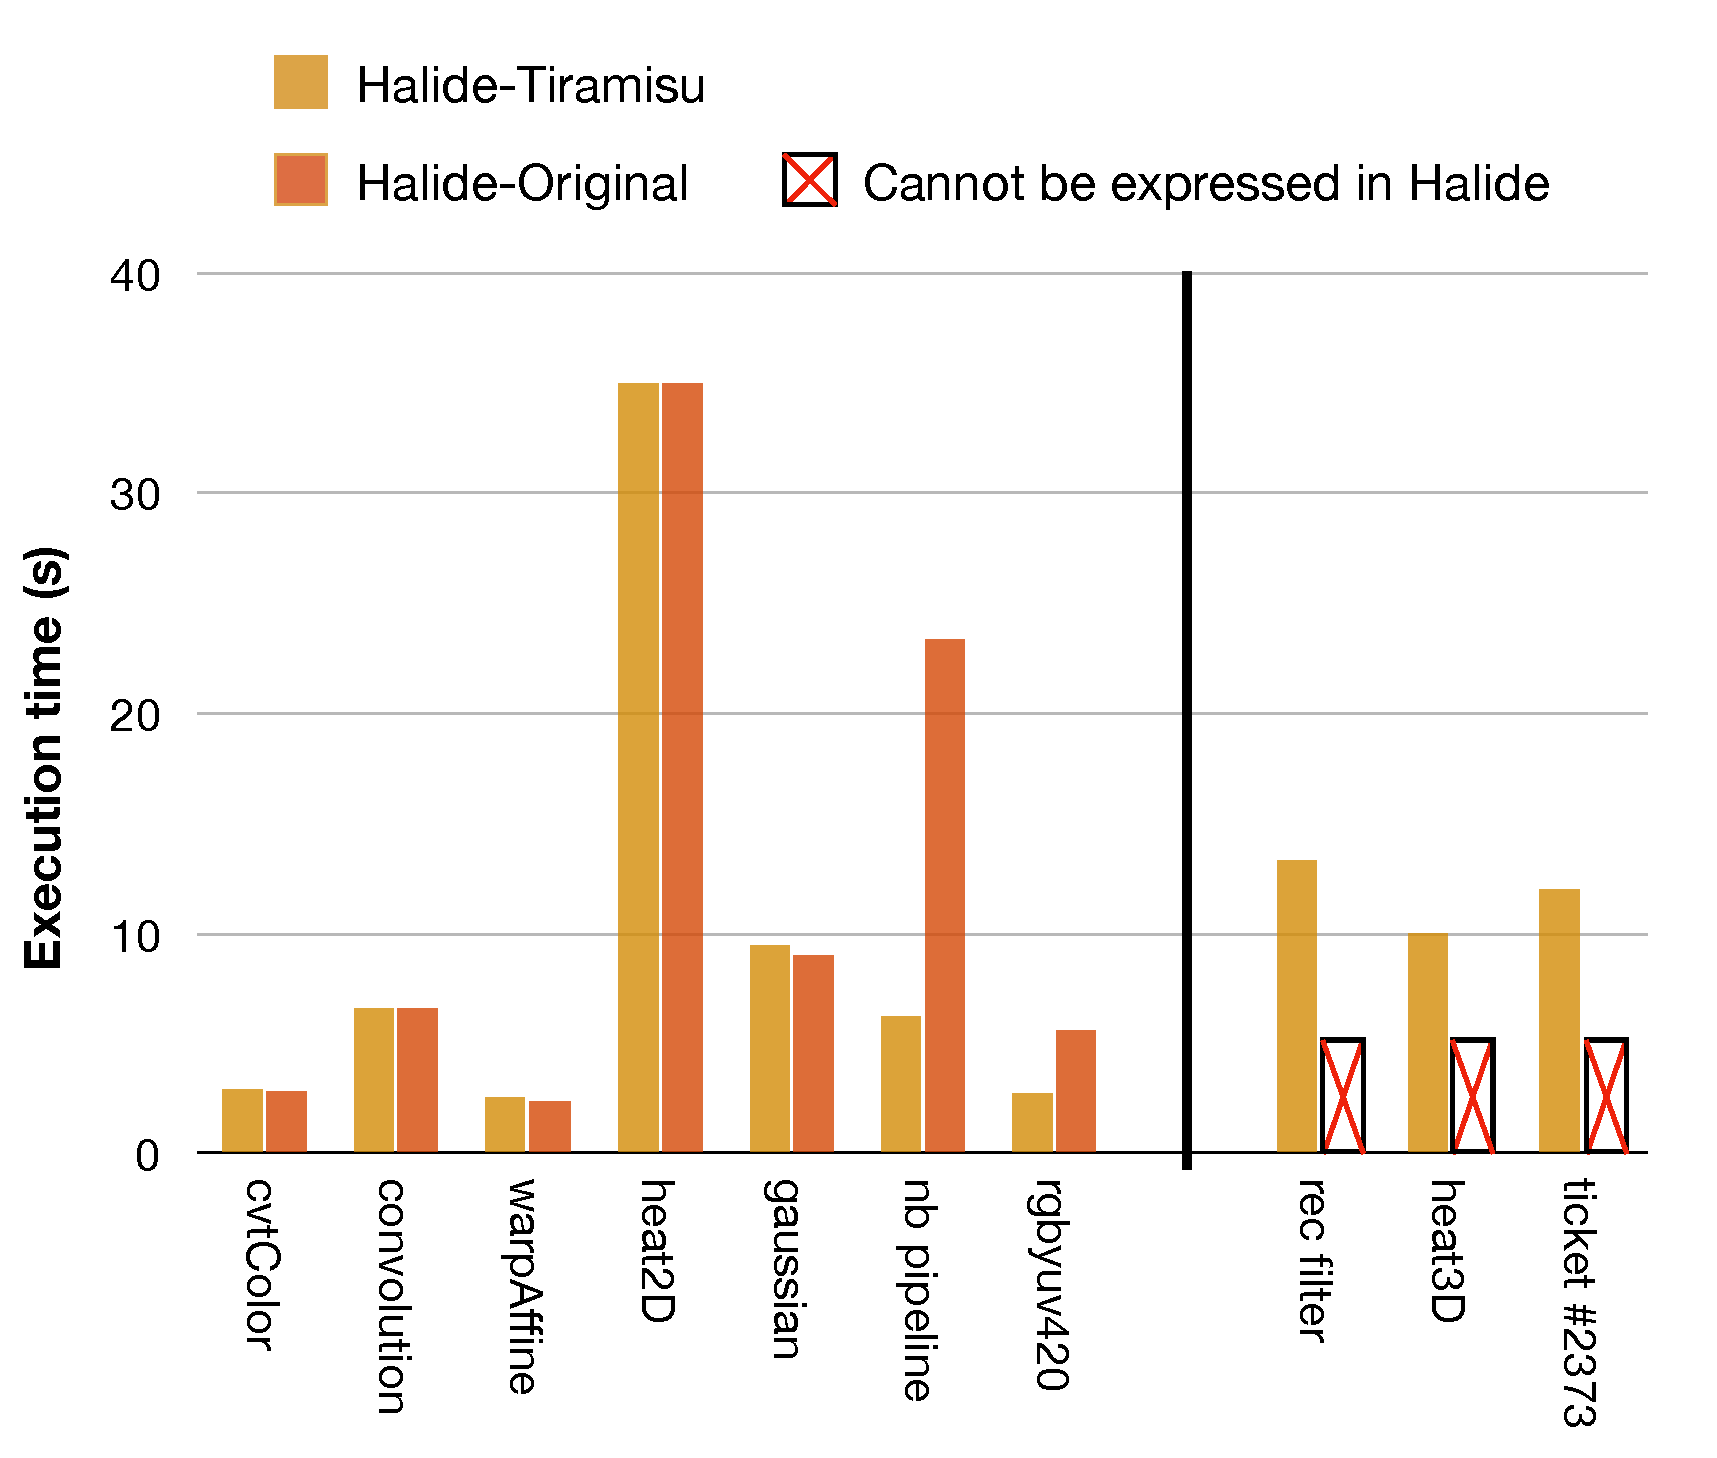
\includegraphics[scale=0.5]{./figures/perf.pdf}
 \caption{Speedup of \framework over Halide}
 \label{fig:speedup}
\end{figure}

We implemented each one of the image processing benchmarks in Halide.  We compile these benchmarks using the original Halide compiler and measure the execution time (we call this compiler Halide-original), then we compile the benchmarks using a modified version of the Halide compiler which uses the \framework framework and measure the execution time (we call this compiler Halide-\framework).  We report the speedup of code generated by the Halide-\framework compiler over the code generated by the Halide-original compiler; the baseline is the Halide-original compiler.

Figure~\ref{fig:speedup} shows the speedups of the \framework framework over Halide.
In three of the benchmarks (\emph{Color conversion}, \emph{2D convolution} and \emph{Recursive Filter}), the performance of the code generated by Halide-\framework matches the performance of the Halide-original.  The same schedule used within Halide-original is generated and used within Halide-\framework.  

The \emph{Recursive Edge Detector} benchmark cannot be implemented in Halide given that it has a recursive definition (Halide does not allow recursive definitions).  Thus we implement the baseline for this benchmark in C rather than Halide.  That C code has two loop nests, the two loop nests can be parallelized but such a parallelism does not provide the best data locality.  In order to get both parallelism and data locality, we need to exploit wavefront parallelism by skewing the iteration space.  Expressing skewing in Halide is challenging since Halide uses an interval based representation in which expressing skewing is not trivial.  The \framework framework uses a polyhedral-based representation that is more expressive than the interval based representation used within Halide and thus \framework can easily express and apply skewing.
When we apply skewing in \framework, the code generated by Halide-\framework is $10.5\times$ faster than the sequential C code and is $2.7\times$ faster than the parallel C code (parallelization without skewing).  This benchmark shows that skewing in this case is good for performance since it enhances both data locality and
parallelism.
The benchmark also provides an example of a complex quasi-affine transformation of the iteration space that is not currently supported by Halide.  This shows the ability of \framework to express complex affine loop nest transformations.

In the last benchmark, \emph{Filter Pipeline}, we have two loop nests that both consume the same image.  Fusing these two loop nests enhances data locality but loop fusion is not currently supported in Halide.  With fusion, we get $3.8\times$ speedup over the non fused Halide code.

\begin{figure}
\centering
 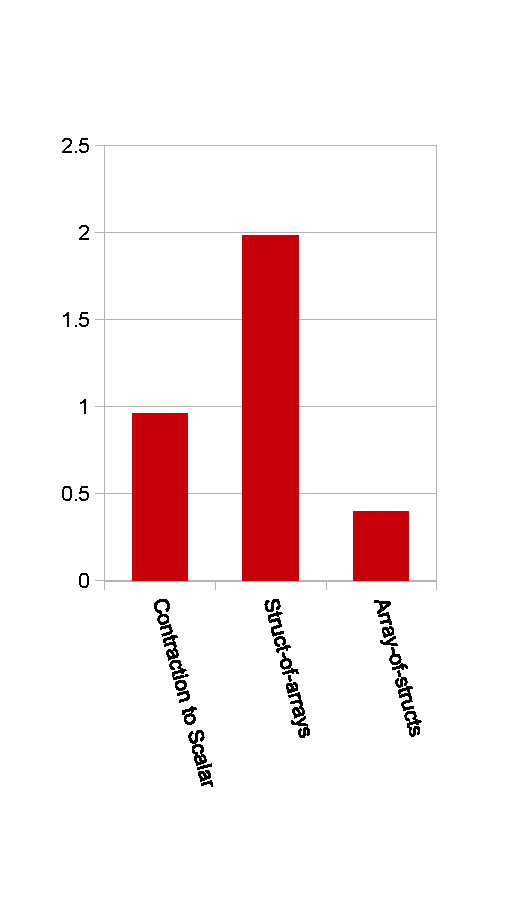
\includegraphics[scale=0.7]{./figures/perf2.pdf}
 \caption{Speedup of \framework over Halide for different data-layouts in an image processing pipeline}
 \label{fig:speedup2}
\end{figure}

Figure~\ref{fig:speedup2} shows the speedup of code generated from Halide-\framework over code generated from Halide-original for different data layouts.  We map the computations of an image processing pipeline to three different data-layouts: full contraction to scalars, struct-of-arrays and array-of-structs.  The goal of this experiment is not to evaluate the gains in performance but rather to show that \framework can actually perform data-layout transformations such as mapping to SOA, AOS and contraction.

\subsection{Integrating \framework into Julia}



\subsection{Integrating \framework into Theano}


\subsection{Tiramisu Code Generators}


Overall, the experiments demonstrated the use of \framework as an IR and an optimization framework for an industrial-strength DSL.  It showed that our implementation matches Halide without losing performance.  In addition, it showed that the three-layer representation allows us to perform advanced loop nest transformations such as skewing which cannot be done in Halide.
The experiments also show that \framework can map computations to different data layouts successfully. % It is up to the user to choose the right data-layout though.


\vspace*{-0.25cm}
\section{Related Work\label{related}}
\vspace*{-0.1cm}
\paragraph{Polyhedral compilers with automatic scheduling.}

Polyhedral compilers such as PENCIL~\cite{pencil,pencil_paper}, Pluto~\cite{bondhugula_practical_2008}, Polly~\cite{polly}, Tensor Comprehensions~\cite{Vasilache2018TensorCF}, and PolyMage~\cite{Mullapudi:2015:PAO:2786763.2694364} are fully automatic.  Some of them are designed for specific domains (such as Tensor Comprehensions and PolyMage), while Pluto, PENCIL, and Polly are more general.
While such fully automatic compilers provide productivity, they may not always obtain the best performance.  This is due to many reasons: first, these compilers do not implement some key optimizations such as array packing~\cite{Goto:2008:AHM:1356052.1356053}, register blocking, data prefetching, and asynchronous communication (which are all supported by \framework{}); second, they do not have a precise cost-model to decide which optimizations are profitable.  For example, the Pluto~\cite{bondhugula_practical_2008} automatic scheduling algorithm (which is used for automatic scheduling in Pluto, PENCIL, Polly, and Tensor Comprehensions) tries to minimize the distance between producer and consumer statements while maximizing outermost parallelism, but it does not consider the data layout, redundant computations, or the complexity of the control of the generated code.  PolyMage uses a custom scheduling algorithm designed for image processing code, but such an algorithm does not address all the complexities that arise when targeting GPUs and distributed systems.
Instead of fully automatic scheduling, \framework uses a more pragmatic approach and relies on a set of scheduling commands, giving the user full control over scheduling.

% and to map buffers to the right memory hierarchy level; it needs to decide about the correctness of non-affine and data-layout transformations; it needs ; and it needs a sophisticated search technique to search efficiently the very large space of optimizations.  

Polyhedral frameworks proposed by ~\citet{Amarasinghe:1993:COC:173262.155102} and~\citet{6877466} address the problem of code generation for distributed systems. \framework{} makes a different design choice, relying on the user to provide scheduling commands to control choices in the generated code (synchronous/asynchronous communication, the granularity of communication, buffer sizes, when to send and receive, the cost of communication versus re-computation, etc.).

Even though \framework{} focuses on providing mechanisms for code optimization, it is still possible to build a framework that provides policy on top of \framework{} (i.e., a framework that automates scheduling).  This separation provides flexibility, making it possible to plug in different policies depending on user requirements.  %The separation between mechanism and policy allows users to choose between using automatic scheduling or manual scheduling which provides more flexibility.

%\vspace*{-0.3cm}
\paragraph{Polyhedral compilers with a scheduling language.}
AlphaZ~\cite{yuki2012alphaz}, CHiLL~\cite{chill,Hall2010}, URUK~\cite{Girbal2006}, and Transformation Recipes~\cite{Hall:2009:LTR:2155247.2155251} are polyhedral frameworks and methods developed to allow users to express high-level transformations using scheduling commands. 
Since these frameworks are polyhedral, they can express any affine transformation.
Their scheduling languages do not target distributed architectures, however, nor do they target GPUs (except the Transformation Recipes framework).  In comparison with these frameworks, \framework features scheduling commands for partitioning computations for execution on a distributed system, synchronization, distribution of data across nodes, mapping data to specific GPU memory hierarchy levels, and performing array packing.  The first four columns of Table~\ref{tab:related} show a summary of a comparison between \framework{} and three representative polyhedral frameworks.

\begin{table}[tb]
    \scriptsize
    \setlength\tabcolsep{1pt}
    \begin{tabular}{l|l|l|l|l|l}
        \hline
        
        \textbf{Feature} & \textbf{Tiramisu} & \textbf{AlphaZ} & \textbf{PENCIL} & \textbf{Pluto} & \textbf{Halide} \\\hline

        \textbf{CPU code generation} & \yes & \yes & \yes & \yes  & \yes \\\hline

        \textbf{GPU code generation} & \yes & \no & \yes & \yes  & \yes \\\hline

        \textbf{Distributed CPU code generation} & \yes & \no & \no & \yes  & \yes\\\hline
        
        \textbf{Distributed GPU code generation} & \yes & \no & \no & \no  & \no\\\hline

        \textbf{Support all affine loop transformations} & \yes & \yes & \yes & \yes  & \no\\\hline

        \textbf{Optimize data accesses} & \yes & \yes & \no & \no & \yes \\\hline

        \textbf{Commands for loop transformations} & \yes & \yes & \no & \no & \yes\\\hline

        \textbf{Commands for optimizing data accesses} & \yes & \yes & \no & \no & \yes \\\hline

        \textbf{Commands for performing data copies} & \yes & \no & \no & \no & \no \\\hline

        \textbf{Commands for memory hierarchies} & \yes & \no & \no & \no & \limited\\\hline

        \textbf{Expressing cyclic data-flow graphs} & \yes & \yes & \yes & \yes & \no \\\hline

        \textbf{Support non-rectangular iteration spaces} & \yes & \yes & \yes & \yes & \limited\\\hline

        \textbf{Instance-wise, exact dependence analysis} & \yes & \yes & \yes & \yes  & \no\\\hline
        
        \textbf{Compile-time affine-set emptiness check} & \yes & \yes & \yes & \yes  & \no\\\hline

        \textbf{Implement support for parametric tiling} & \no & \yes & \no & \no  & \yes\\\hline
    \end{tabular}
    \caption{Comparison Between Different Frameworks.}
    \label{tab:related}
    \vspace{-0.75cm}
\end{table}

\paragraph{Non-polyhedral compilers with a scheduling language.}
Halide~\cite{halide_12} is an image processing DSL that has a scheduling language; however, it uses intervals to represent iteration spaces instead of the polyhedral model.  This limits the expressiveness of Halide.
For example, Halide cannot naturally represent non-rectangular iteration spaces.  This makes certain Halide passes over-approximate non-rectangular iteration spaces, potentially leading to less efficient code.  It also makes Halide over-approximate the amount of data to communicate (send and receive) when generating distributed code,  and also prevents Halide from performing precise bounds inference for non-rectangular iteration spaces, as well as performing many complex affine transformations, such as iteration space skewing, which are all possible in \framework{}.

Halide does not have dependence analysis and thus it relies on conservative rules to determine whether a schedule is legal; for example, Halide does not allow the fusion of two loops (using the \texttt{compute\_with} command) if the second loop reads a value produced by the first loop.
While this rule avoids illegal fusion, it prevents fusing many legal common cases which may lead to suboptimal performance.
Halide also assumes the program has an acyclic dataflow graph in order to simplify checking the legality of a schedule. This prevents users from expressing many programs with cyclic dataflow.
It is possible in some cases to work around the above restrictions, but such methods are not general.
\framework{} avoids over-conservative constraints by relying on dependence analysis to check for the correctness of code transformations, enabling more possible schedules.  Table~\ref{tab:related} shows a comparison between \framework{} and Halide.

Other systems include POET~\cite{Yi:2007ay}, which uses an XML-based description of code and transformation behavior to parametrize loop transformations.  It uses a purely-syntactic transformation system to produce transformed code.  The use of syntactic transformations is less general than the polyhedral model used in \framework.

\paragraph{Non-polyhedral compilers with automatic scheduling.}

Delite \cite{chafi_domain-specific_2011} is a generic
framework for building DSL compilers using Lightweight Modular Staging (LMS) \cite{lms_staging_10}. It exposes several parallel computation patterns that DSLs can use to express parallelism.
NOVA~\cite{Collins:2014:NFL:2627373.2627375} and Lift~\cite{Steuwer:2017:LFD:3049832.3049841} are other IRs for DSL compilers.  They are functional languages that rely on a suite of higher-order functions such as map, reduce, and scan to express parallelism.
Weld~\cite{palkar2017weld} is another IR designed for the area of databases and data analytics and can be used to implement libraries, such as Numpy~\cite{numpy}, and enable optimizations across different library calls.
\framework{} is complementary to all of these frameworks as \framework{} would allow them to perform and compose a large set of complex affine transformations that are easier to express in the polyhedral model.

%The Cyclops Tensor Framework (CTF)~\cite{solomonik2013cyclops} is a library for performing tensor contractions, primarily in the field of quantum chemistry. CTF automatically decomposes tensors using a communication-optimal tensor contraction algorithm and maps the computations to the underlying architecture. The framework targets distributed architectures, and can provide hybrid execution through the use of MPI and OpenMP.  Unlike \framework{} which is designed to be more general, CTF is designed mainly for tensor contractions.
%Chapel~\cite{Chamberlain:2007:PPC:1286120.1286123} is a parallel programming language that supports a Partitioned Global Address Space (PGAS) memory model~\cite{Krishnamurthy:1993:PPS:169627.169724}.  In this model, code can refer to variables and arrays regardless of whether they are stored in a local or remote memory.  Any necessary communication is automatically inserted by the compiler and executed at runtime.  Similarly, computations in Layer I of \framework{} refer to other computations in the same way regardless of whether they are stored or computed in local or remote memory (or in shared or global memory on GPU).  Specifying whether a computation is local or remote, how it is accessed and whether communication is needed are all done using scheduling commands at Layers II, III and IV. \framework{} provides a set of fine-grain commands that can implement any data-mapping and communication that a language like Chapel provides, yet \framework{} can complement Chapel by providing new capabilities such as advanced loop nest transformations and checking schedule validity.
% large has the advantage of enabling manual scheduling, data mapping and communication (while Chapel.


\section{Conclusion and Future Work}

In this paper we introduce \framework, a mid-end compiler for domain specific languages that separates the algorithm, the schedule and the data layout.
\framework has a three-layer intermediate representation that enables the separation.  The first layer of the IR describes computations without describing how these computations are scheduled or where the intermediate values are stored.  The second layer describes how computations are scheduled but does not represent where the values are stored.  The third layer specifies data layout.

\framework{} provides three methods to generate Layer II and Layer III.  The first method is a set of transformation primitives, similar to the primitives used in Halide~\cite{halide_12} or ChiLL~\cite{chill}. The second method is the direct generation of Layer II and Layer III.
The third method is a quasi-affine schedule (map) that transforms the set of computations in Layer I into a set of computations in Layer II.

We evaluate \framework by creating a new middle-end for the Halide compiler, and demonstrate no loss of performance.  Finally, we also demonstrate transformations made possible by \framework that are not possible in Halide such as skewing and fusion, increasing performance by up to $10\times$.

Future work includes support for more DSL compilers and adding a layer of automation on top of the current framework; for example, we want to enable automatic scheduling within \framework.



%% -------------------------------------------------

% \acks

% Acknowledgments, if needed.

% We recommend abbrvnat bibliography style.

%% -------------------------------------------------


\bibliographystyle{abbrvnat}

% The bibliography should be embedded for final submission.

\bibliography{bibliography}

%\appendix
%\section{Appendix: Definitions}

\end{document}



%%%% Archive for text removed from the paper (if needed later)
%%%%%%%%%%%%%%%%%%%%%%%%%%%%%%%%%%%%%%%%%%%%%%%%%%%%%%%%%%%%%%%%%%%%%%%%%

%\framework uses an expressive representation for the three levels of the IR based on the polyhedral model; The separation between the three-levels is designed not only to separate computations from the schedule and data-layout specifications but also to open the door for affine transformation frameworks to work in synergy with non-affine transformation frameworks.  This is mainly because the transformation from one IR level to another can be done using an affine transformation or a non-affine transformation framework.  Code generation is unified, whether an affine or a non-affine transformation framework is used.

%%%%%%%%%%%%%%%%%%%%%%%%%%%%%%%%%%%%%%%%%%%%%%%%%%%%%%%%%%%%%%%%%%%%%%%%%

\begin{comment}

\subsection{Integrating Affine and Non-affine Transformations in one Framework}

An extensive amount of research has been done in the area of polyhedral compilation and affine program transformations~\cite{}.  Polyhedral compilation uses an abstract mathematical representation to model programs: the iteration domain of a statement is represented as a set described using affine constraints (linear constraints) while loop transformations are expressed using affine relations between the iteration domain and a time domain.  Although such a representation is very expressive and can express affine transformations such as non-parametric loop tiling, loop fusion, loop distribution, loop skewing, ... little attention has been given to the integration of affine transformation frameworks with non-affine transformation frameworks (which can express non-affine transformations such as parametric tiling, parametric splitting, ...).

In this paper, we introduce a common representation that can be used by both frameworks.  It is hybrid representation that combines the expressiveness of the polyhedral representations with the generality of interval based representations.  Transformations are still done in separate frameworks but the representation of the iteration domain, the time-space domain and the data-domain is unified.  We use one code generator to generate code in both cases.  We believe that such a representation is the right level of abstraction that can opens the door for polyhedral and affine-transformation frameworks to work in synergy with non-affine transformation frameworks.  This allows \framework to perform advanced transformations that are difficult to perform for a non-affine framework yet it can apply many classes of non-affine transformations.

\subsection{Contributions}

\framework is a intermediate representation and an open source framework for advanced iteration space transformations. It supports affine transformations and some classes of non-affine transformations.  The paper introduces:
\begin{itemize}
  \item A three-level IR that separates the algorithm from the schedule and the data-layout.  The first level describes the computations without describing how these computations are scheduled or where they are stored.  The second level describes how computations are scheduled but does not represent how they are stored.  Since this level does not represent the memory-layout, reasoning about code transformations becomes easier, since code transformation passes do not need to transform the data layout.  The third level specifies the data-layout.
  \item A hybrid representation for the iteration domain and the time-space domain; this representation is based on integer intervals and on integer sets described with affine constraints.
  \item A code generator that takes as input the hybrid time-space representation (which is a combination of integer intervals and affine constraints) and generates as output a sequence of loop nests.
  \item The framework allows the application and the composition of affine transformations as well as some classes of non-affine transformations.
  \item An open source framework that implements the three-level IR and generates code targeting single core CPU, multi-core CPU with vectorization and targets GPU architectures.  This level is validated on the Halide DSL industrial compiler.
\end{itemize}

%\begin{itemize}
%  \item A three-level IR that separates the algorithm from the schedule and the data-layout. Since the memory-layout is not represented in the high levels of the IR where scheduling happens, reasoning about code transformations is easier since it does not involve data-layout transformations as well.
  %, since code transformation passes do not need to transform the data layout.  The third level specifies the data-layout.
  %The first level describes the computations without describing how these computations are scheduled or where they are stored.  The second level describes how computations are scheduled but does not represent how they are stored.  
%  \item The framework allows the user to use an affine transformation or a non-affine transformation to transform the iteration domain to the time-space domain.
%  \item A code generator that takes as input the time-space representation regardless of whether it was generated using an affine or a non-affine transformation; it generates a sequence of loop nests as output.
%  \item An open source framework that implements the three-level IR and generates code targeting single core CPU, multi-core CPU with vectorization and targets GPU architectures.  This framework is validated on the Halide industrial DSL compiler.
%\end{itemize}

%%%%%%%%%%%%%%%%%%%%%%%%%%%%%%%%%%%%%%%%%%%%%%%%%%%%%
%To illustrate this workflow, let us take the following code that implements a $3\times3$ box filter defined as two $3\times1$ filters.

%\begin{lstlisting}[language=C,basicstyle=\scriptsize]
%for (x in 0..N)
% for (y in 0..M)
%  blurx(x,y) = (in(x-1,y) + in(x,y) + in(x+1,y))/3
%for (x in 0..N)
% for (y in 0..M)
%  blury(x,y) = (blurx(x,y-1) + blurx(x,y)+blurx(x,y+1))/3
%\end{lstlisting}

%The first computation, blurx, computes a horizontal blur of the input by averaging over a $3\times1$ window and the second computation, blury, computes the final blur by averaging a $1\times3$ window of the output from the first computation.

% Let us suppose that we want to perform 


%%%%%%%%%%%%%%%%%%%%%%%%%%%%%%%%%%%%%%%%%%%%%%%%%%%%%%

\begin{figure}[h]
\begin{lstlisting}[language=C,basicstyle=\scriptsize]
for (i in 0..N)
  for (j in 0..M)
    y(i,j) = 66*rgb(i,j,0) + 129*rgb(i,j,1) + 25*rgb(i,j,2)
for (i in 0..N)
  for (j in 0..M)
    u(i,j) = -38*rgb(2*i,2*j,0) - 74*rgb(2*i,2*j,1) + 112*rgb(2*i,2*j,2)
for (i in 0..N)
  for (j in 0..M)
    v(i,j) = 112*rgb(2*i,2*j,0) - 94*rgb(2*i,2*j,1) - 18*rgb(2*i,2*j,2)
for (i in 0..N)
  for (j in 0..M)
    consumer(i,j) = y(i,j) + u(i,j) + v(i,j)
\end{lstlisting}
\caption{\label{fig:rgb2yuv1} RGB to YUV}
\end{figure}

\end{comment}